\documentclass[12pt,english]{article}
\usepackage[T1]{fontenc}
\usepackage{mathptmx}
%\renewcommand{\familydefault}{\sfdefault}
\usepackage[latin9]{inputenc}
\usepackage{multirow}
\usepackage{multicol}
\usepackage[letterpaper]{geometry}
\geometry{verbose,tmargin=3.8cm,bmargin=3.8cm}
\usepackage{float}
\usepackage{amstext}
\usepackage{amsmath}
\usepackage{mathptmx}
\usepackage{amsthm}
\usepackage{array}
\usepackage[capposition=top]{floatrow}

\newtheorem{hypothesis}{Hypothesis}
\usepackage[title,titletoc]{appendix} 
\usepackage{multirow}
\newtheorem{result}{Result}
%\usepackage{theorem}
\newtheorem{hypo}{Hypothesis}
\usepackage{harvard}
\usepackage{graphicx}
\usepackage{ amssymb }
\usepackage{url}
\usepackage{epstopdf}
\usepackage{caption}
\usepackage{subcaption}
\usepackage{natbib}

\graphicspath{{figures/}}

\usepackage{setspace}
\usepackage{esint}
\onehalfspacing
\usepackage{babel}
\DeclareMathOperator*{\med}{med}

\hyphenation{parti-cularly}

\begin{document}

\title{Gender differences in an endogenous timing conflict game }

\author{Philip J. Grossman
\thanks{Department of Economics, Monash University}\thanks{Corresponding Author. \textit{Email:} Philip.Grossman@monash.edu \textit{Address:} Level 8, Robert Menzies Building. Scenic Blvd \& Wellington Road, Clayton VIC 3800, Australia.} \and Youngseok Park\thanks{Department of Economics, Colby College} \and Jean Paul Rabanal
\footnote{Department of Banking and Finance, Monash University} \and Olga A. Rud \footnote{Department of Economics, RMIT Univeristy} }\date{\today}
\maketitle
\begin{abstract}
We conduct a laboratory experiment to study the role of gender on social welfare outcomes in a strategic commitment game of incomplete information. In our baseline treatment, players simultaneously commit to either a Hawkish action or a Dovish action, which can enhance social welfare. We add a sequential and an endogenous move treatment, where in the former, the first mover is exogenously selected and in the latter, players self-select the order of play. We find that (i) social welfare is significantly improved in the last two treatments and (ii) men are more willing to play Dove in the endogenous treatment.

%We conduct a laboratory experiment to study the role of gender on social welfare outcomes in a strategic commitment game of incomplete information. In our baseline treatment, players simultaneously commit to either a Hawkish action, which leads to a private payoff, or a Dovish action, which can enhance social welfare. We add a sequential and an endogenous move treatment, where in the former, the first mover is exogenously selected and in the latter, players self-select the order of play. The two additional treatments relax the commitment constraint for the second mover. We find that (i) social welfare is significantly improved in the last two treatments and (ii) the outcome in the endogenous move treatment is mainly driven by gender. Men are willing to play the risky Dovish action more often than women. 
\end{abstract}
\textbf{Keywords:}
gender; type uncertainty; endogenous timing; laboratory experiment\\
\textbf{JEL codes:} C72, C92, D82, D91
\newpage
\section{Introduction}
\label{sec:intro}

Recent evidence suggests that women are willing to volunteer more often than men when their incentives align with the social welfare (Babcock et al., 2017). However, in some cases, socially optimal behavior could be undermined due to lack of commitment. This occurs when a socially optimal choice is perceived as risky by players who are increasingly uncertain in counterparty behavior.\footnote{Thomas Schelling's ideas on the role of commitment on social welfare outcomes have motivated a number of studies in non-cooperative game theory as well as in experimental economics. Hamilton and Slutsky (1990), Maliath (1993), and Normann (2002) in duopoly games; Andreoni (1998) in public goods;  Dasgupta (2007) and Farrell and Saloner (1985) in coordination games; and Baik and Shogren (1992) in contest games. Experimental work related to games of complete information (based on Hamilton and Slutsky, 1990), examined the emergence of Stackelberg leadership in duopoly games (strategic substitutes) where players set quantities. Evidence (Huck et al. 2001, 2002) suggests that Cournot and other collusive outcomes appear more often than theory predicts.} Therefore, how a risk profile of the same strategy set is evaluated by gender can become extremely salient in determining social welfare outcomes in games of incomplete information.

The fear of choosing the socially optimal action due to uncertainty about counterparty type is an interesting feature of a two-player game first introduced by Baliga and Sj\"ostr\"om (2004, hereafter BS04). BS04 present a simultaneous-move game where players are uncertain about the counterparty's payoff for playing an aggressive action, hawk ($H$). In their environment, the payoff to each player for choosing $H$ depends on player type. Hence, some players have more incentive to play $H$ compared to others. Furthermore, the incentive to choose dove ($D$), the socially optimal action, is positively correlated with the belief that the counterparty will reciprocate.\footnote{This feature is known as strategic complementarity. BS04 also study strategic substitutes, which we omit in the present paper.} The incentive structure in our paper is different than in Babcock et al. (2017), who focus on a volunteer game with strategic substitutes and find that women switch from $H$ to $D$ more often compared to men.\footnote{The model in BS04 can also be analyzed using a population game. For example, consider the voluntary contributions game with subjective idiosyncratic costs of contributing in a population analyzed in Rabanal (2017) who adopts gradient and replicator dynamics, respectively.}

Building upon the framework of BS04, we incorporate an additional layer of uncertainty by varying how the order of play under action commitment is determined. We design this experiment to study whether gender differences are important for achieving a social optimum in the presence of uncertainty. In our baseline treatment, $CGO$, we replicate the simultaneous move environment of BS04. Our two new treatments, which we formally analyze below, propose (i) an exogenously determined, sequential-move game, $CGS$, which controls for the strategic uncertainty associated with non-simultaneous order of play, and (ii) an endogenously determined (self-selected) order of play, $CGE$, which can result in two distinct games. The $CGE$ treatment can lead to a simultaneous-move game when both players choose the same order of play, or a sequential-move game when players have varying preferences for order of play. Uncertainty about the environment can make the choice to play $D$ risky relative to the $CGS$ environment, where a player knows with certainty that the game will be sequential in nature. However, in both the $CGS$ and $CGE$ treatment, the commitment to a strategy selected in the first stage of the game is non-binding for the second mover (i.e. when the game is sequential in either treatment). This allows for a strategic response, which should imitate the action of the first player. Specifically, for a wide family of player types, the first mover can set the stage by playing $D$ and incentivize the second player to reciprocate. Selection of $D$ by both players leads to the socially optimal outcome.

To help subjects choose when to play $H$ or $D$, we implement a cutoff strategy using a slider which asks for a minimum required payoff to play $H$.\footnote{A similar cutoff elicitation task, but without a slider, also appears in Duffy and Ochs (2012). They find that the elicited cutoff is consistent with the actual binary choices in their entry game. Additionally, Van Huyck et al. (2018) survey the participants about how they play the game. Seventy two percent report using a threshold. Similar to the behavior observed in our experiment, Duffy and Ochs (2012) also find that there is a significant variation in cutoff strategies across subjects.} The private payoff realization (which we draw based on a uniform distribution) defines the commitment strategy for the first mover in the $CGS$ and $CGE$ treatments, and for all players in a simultaneous-move game in the $CGO$ and $CGE$ treatments. Note that players in the $CGS$ treatment do not know if they are first or second movers when they decide a cutoff strategy. However, they are aware that the decision is not binding if they are second movers which occurs with 50 percent probability. Thus, the uncertainty of being first or second mover does not affect the cutoff decision which is only relevant for the first mover.

Experimental results show that in the $CGS$ treatment both men and women increase their cutoff relative to the $CGO$ treatment in the direction predicted by theory, but not to the extent assumed by risk neutrality. Playing $D$ can be risky given the possible payoff loss of 95 percent should the second mover be revealed a hawk-dominant type (10 percent chance). Instead, by playing $H$, the first mover is guaranteed a minimum payoff (determined by the cutoff strategy), and can earn more if the second mover is a dove-dominant type (5 percent chance). Overall, the frequency of $DD$ (the social optimum) in the $CGS$ treatment is 20 percentage points higher relative to the $CGO$ treatment. 

 Important gender differences emerge in the presence of environmental uncertainty in the $CGE$ treatment. Women appear to follow the cutoff strategy that is similar to the one observed in the $CGO$ treatment, and evenly distribute their preferred order of play across both periods. Men, on the other hand, select a cutoff strategy that is similar to the one observed in the $CGS$ treatment and strongly prefer to move second. In the $CGE$ treatment, half of all encounters between subjects result in a sequential game, one third in a simultaneous game played in the second period and the rest, in a simultaneous game played in the first period. Remarkably, the frequency of $DD$ play is similar across the $CGE$ and $CGS$ treatments.

Furthermore, our results suggest that strategic uncertainty may undermine cooperation by women in establishing a Pareto superior outcome (e.g. see Babcock et al., 2017). Lack of cooperation has been observed in situations where women appear to be more averse to the ``sucker" effect, which occurs when individuals free-ride because they believe that others will as well (see Ingram and Berger, 1977; and Van den Assem et al., 2012). A recent lab-in-the-field experiment in rural India by Gangadharan et al. (2018) finds that women as leaders contribute less than what they proposed in a public good game, which may suggest that women fear being the ``sucker." 


In a survey paper on gender risk attitude, Niederle (2016) finds that while differences in preferences exist, they vary considerably depending on the elicitation method. Our results also appear to support this notion. In the $CGO$ and $CGS$ treatments, women approach risk in a similar fashion to men. That is, we do not observe any differences in behavior across gender. However, when the order of play is endogenously determined, a gender difference appears. Our experimental design does not reveal to the subjects that we aim to measure gender differences. All sessions are roughly gender balanced in composition.\footnote{We attempted to recruit balanced sessions. Our final data set includes marginally more (less) women in the $CGO$ and $CGS$ ($CGE$). Please see Table \ref{session} for more details.}

Our paper is related to previous experiments that study cutoff strategies in games of incomplete information with strategic complements.\footnote{For a theoretical description of pre-commitment in games of complete information with strategic complements and/or substitutes, please refer to Eaton (2004).} Brindisi et al. (2014) find that in an investment game with correlated player types (a joint investment opportunity), endogenous timing improves social welfare. Specifically, the results suggest that coordination is higher under endogenous timing, though it is still lower than predicted. In the simultaneous-move game, subjects use a cutoff strategy that deviates from theory, and approaches payoff dominance which is similar to what we observe in the $CGO$ treatment. Other games of incomplete information (Van Huyck et al., 2018) and complete information (Heinemann et al., 2004 and Duffy and Ochs, 2012) also report similar findings. However, for some simultaneous move games of incomplete information, risk dominance becomes an important factor in strategy selection (Cabrales et al., 2007).

According to the experimental results of Heggedal et al. (2018), risk aversion can deter a first mover from committing to an irreversible action. Their study tests the main predictions of Farrell and Saloner (1985), which is closely related to the environment of BS04. In stage one, players simultaneously decide whether to: (i) remain at status quo (known payoffs) or (ii) choose an alternative (risky payoff) that is irreversible. In stage two, only those players who have not yet committed choose between the two alternatives. If no player committed in stage one, second stage decisions become simultaneous. The results show that, when the risk of failure is low, players are willing to commit and that they follow the equilibrium cutoff strategy. When the risk of failure is high (i.e. a large payoff loss if the other does not follow up) players are less willing to commit and the behavior deviates from the theoretical prediction. These findings are similar to what we observe in the $CGS$ treatment and partly in the $CGE$ treatment. In addition, our results also suggest that men are more willing than women to accept the risk of failure (or success).\footnote{There is  mixed evidence regarding gender differences in other contest games or tasks. For example, in winner-pay common value (Casari et al., 2007; Ham and Kagel, 2006), first-price auction (Chen et al., 2013) and all-pay auction (Chen et al., 2015) there is robust evidence that women bid more aggressively than men. In real effort tasks, losses deter women but not men from competition (Gill and Prowse, 2004). When the stakes of the test are low, female students perform better than male students, but the gap across students decreases as the stakes increase (Azmat, et al., 2016). Jetter and Walker (2018), using data from Jeopardy!, find that women compete more aggressively and take on more risk when paired against men.} 

Our paper is also related to other gender literature which studies coordination games under strategic complements. Similar to our $CGO$ and $CGS$ results, these studies do not find significant gender differences.  Dufwenberg and Gneezy (2005) compare the performance of men and women in a repeated, minimum-effort coordination game where the gender composition of teams was not announced (single gender) but participants could observe other players. The study found no significant difference in chosen effort. Di Girolamo and Drouvelis (2015) analyze the performance of single-gender and mixed-gender groups in the same game as Dufwenberg and Gneezy (2005). In the single-gender treatment, subjects know the gender of their team members; in the mixed-gender treatment, subjects are unable to discern the gender mix of their team. Di Girolamo and Drouvelis also found no significant differences in chosen effort. Similarly, in a coordination game with strategic complements, Heinemann et al. (2009) find no observable gender difference.\footnote{In a different environment, studying the effect of gender on leader/group choices, Grossman et al. (2015) find that women leaders are more willing to take risks in an investment game (strategic substitutes) when playing in single-gender groups or in mixed gender-groups and their gender was not revealed to their responders. The responders, on the other hand, behave similarly regardless of the leader's gender.}

\section{The conflict game}
\label{sec:model}
We model our environment after the simultaneous move two-player conflict game of BS04. In this game of incomplete information, player $i$ can pursue either a hawkish (aggressive) action ($H$), or a dovish (peaceful) action ($D$). The action space for a player can be specified as $s\in\{H,D\}$, and leads to the following payoff matrix
\begin{equation}
\begin{pmatrix}
x_i & \mu+x_i \\
k-d & k 
\label{t:payoff}
\end{pmatrix}.
\end{equation}
where $k=100$, $\mu=10$ and $d=95$. When both players play $H$, each player receives $x_i$, which is an idiosyncratic private payoff that is independently drawn from a uniform distribution $F\in [0,k]$. Therefore, the idiosyncratic $x_i$ can be thought of as hawk type, where some players are revealed to be more hawkish and thus reap more benefit from action $H$, and some are revealed to be less hawkish and see a lower return to playing $H$. If both players choose the peaceful action $D$, then the payoff to each player is a constant $k$. If player $i$ plays $D$, while player $j\neq i$ plays $H$, then the payoff to player $i$ is $k-d>0$, where $d$ can be considered a cost of a peaceful action when the opponent is aggressive. On the other hand, if player $i$ plays $H$ and player $j\neq i$ plays $D$, then the payoff to player $i$ is $\mu+x_i$, where $\mu (<d)>0$ can be viewed as a marginal benefit of an aggressive action when the opponent is peaceful. 

The Bayesian Nash Equilibrium (BNE) can be characterized as a cutoff strategy, following BS04, such that a player with a payout lower than $x_i\leq\hat{x}_{_{CGO}}$ will play $D$, and $H$ otherwise.  When a player is indifferent between $H$ and $D$, we can find the cutoff as the unique fixed point where 
\begin{equation}
\hat{x}_{_{CGO}}:= k-d + (d-\mu) F(\hat{x}_{_{CGO}}). \label{eq:cgo}
\end{equation}

\noindent Given that $F(\cdot)$ follows a uniform distribution in the space $[0,k]$, the cutoff point can be rewritten as 
\begin{equation}
\hat{x}_{_{CGO}}:= \frac{k\cdot (k-d)}{k-d+\mu}=33. \label{eq:cgosol}
\end{equation}
A possible mechanism for improving welfare in a $CGO$ game is for players to move sequentially. We study an exogenous sequential move game ($CGS$) and an endogenous move game ($CGE$). In the former, the order of play is randomly determined while in the latter players self-select the order of play. Social welfare under a $CGS$ game is significantly higher relative to the $CGO$ game. In a $CGE$ game, social welfare may be similar to either the $CGO$ or a $CGS$ environment. That is, the $CGE$ game can lead to multiple outcomes, which we discuss in greater detail below. We begin by describing the optimal strategy in a $CGS$ game, where a player is randomly selected to move first. 

The cutoff strategy for the first mover in a $CGS$ game shifts to the right of the optimal strategy in a $CGO$ game, such that $\hat{x}_{_{CGO}}\leq\hat{x}_{_{CGS}}$. That is, in order to play $H$, a player in a CGS environment has to be more hawkish, or requires a higher payoff to $H$. The intuition for the rightward shift in the cutoff strategy is fairly straightforward. Consider a first-mover at the original cutoff $\hat{x}_{_{CGO}}$. If the first-mover selects $D$, then she will obtain greater expected profits because the probability that the second mover will play $D$ as well is higher due to strategic complementarity. In other words, the probability that the other player plays $D$ increases from $Pr(x\leq\hat{x}_{_{CGO}}) \equiv F(\hat{x}_{_{CGO}}) $ in the $CGO$ game to  $Pr(\mu+x_j\leq k) \equiv F(k-\mu)  $ in the CGS game. The unique Perfect Bayesian Nash Equilibrium (PBNE) where the first mover uses the cutoff strategy can then be defined as
\begin{equation}
\sigma_i(x_i)=D \quad \text{if} \ \ x_i\leq \hat{x}_{_{CGS}}:= k-\mu=90. 
\end{equation}

\noindent \textit{Proof:} See Appendix A $\blacksquare$

In the CGE game, where the players self-select the order of play, the timing of the game proceeds as follows:

\textit{Stage 0:} Each player $i$ selects a cutoff strategy, indicating a set of values where $\sigma_i(x_i)=H$, and then observes own type $x_i$, but not the other player's type $x_j$ where $j\neq i$.

 \textit{Stage 1:} Both players simultaneously select the period in which to play the game $t=1,2$. 

\textit{Stage 2:} The conflict game is played by the move structure determined in Stage 1. The commitment to the cutoff strategy is not binding for the player $i$ if and only if $t_i=2$ and $t_j=1$. 

The predictions for the $CGE$ game follow the $CGO$ and $CGS$ solutions. Note that if both players select the same time period (e.g. $t=1$), then the environment resembles a simultaneous move game and the equilibrium follows the cutoff strategy specified in BS04. Therefore, in one possible equilibrium, $\hat{x}_{_{CGE}}=\hat{x}_{_{CGO}}=33$ and no player has incentive to deviate. Alternatively, players can coordinate and follow the strategy described in the CGS game, which leads to a different equilibrium where type $x\leq \hat{x}_{_{CGS}}\equiv 90$ will select $t=1$ and commit to $D$, while type $x>\hat{x}_{_{CGS}}$ will wait to play at $t=2$. Again, under this equilibrium players do not have any incentive to deviate. 

\noindent \textit{Proof:} See Appendix A $\blacksquare$
\\

\noindent \textbf{Prediction 1}
\textit{In the simultaneous conflict game ($CGO$) subjects play at or above the cutoff strategy $\hat{x}_{_{CGO}}=33$.}

We reconcile the theoretical solution in the $CGO$ game with experimental evidence for our first prediction. In the laboratory, subjects play $D$ more often than predicted by the Nash Equilibrium (NE). For example, Evdokimov and Garfagnini (2018) find that in the simultaneous move game, subjects play $D$ at a rate of 64 percent compared to 50 percent predicted by theory.\footnote{The main purpose of their study is to test the predictions of Baliga and Sj\"ostr\"om (2012) where a third party can manipulate the two-player conflict game. They find that third party communication is not strategic. Our experiment does not include a third party.}\\ 

\noindent \textbf{Prediction 2}
\textit{The cutoff strategy in the sequential $CGS$ game is higher compared to the cutoff strategy in the simultaneous move $CGO$ game.}

Note that the equilibrium predictions $\hat{x}_{_{CGS}}=90$ and $\hat{x}_{_{CGO}}=33$ are far apart. This allows us to observe meaningful differences even when players chose cutoff values greater than the NE described in Prediction 1. The gain in expected payoff is equal to $d\times \left( F(\hat{x}_{_{CGS}})-F(\hat{x}_{_{CGO}}) \right)=95\times( 90-33)/100=50$ points or 137 percent. \\

\noindent \textbf{Prediction 3}
\textit{\textbf{A.} In CGE, a player will behave as in the $CGO$. } \textit{\textbf{B.} In CGE, a player will behave as $CGS$.}

The $CGE$ environment can lead to multiple equilibria. At this point, we are uncertain about the type of equilibrium that would prevail in our experiment. Two conflicting Predictions, 3A and 3B, reflect our priors. \\

\noindent \textbf{Prediction 4}
\textit{The probability of observing a $DD$ outcome in either the $CGS$ or the $CGE$ game is greater than or equal to the probability of observing the same outcome in the $CGO$ game.}

The coordination required to achieve the $DD$ outcome should be easier to achieve in a sequential game. Therefore, the frequency of $DD$ should be higher in the $CGS$ game compared to the $CGO$ game. The $CGE$ game can lead to two outcomes, which depend on the selected order of play. If players choose the same order of play, then the $CGE$ game should lead to the same outcome as predicted by the $CGO$ game, where $\hat{x}_{_{CGO}}=33$ because the environment will resemble that of simultaneous play. However, if players select distinct time periods, such that $t_i\neq t_j$, then the game is sequential and the prediction becomes similar to one in the $CGS$ environment.  Henceforth, we expect that the frequency of $DD$ under $\hat{x}_{_{CGE}}\geq \hat{x}_{_{CGO}}$$.  \\

\noindent \textbf{Prediction 5}
\textit{There is no gender difference in strategy choices across the three games.}

Even though Babcock et al. (2017) find that women are more accommodating, by choosing to play $D$ more often than men, risk aversion can deter subjects (both men and women) from commitment required to improve social welfare (see Heggedal et al., 2018). We do not take any strong position regarding risk attitudes across gender following Niederle (2016). 


\section{Laboratory procedures}
\label{sec:game}

The experiment was conducted at the Rosario Experimental and Behavioral Economics Lab (REBEL) of the Universidad del Rosario, Colombia. Participants were undergraduate students from all fields and were recruited online via ORSEE (Greiner, 2015). Subjects were part of one of the three treatments (between design) ---$CGO$, $CGS$ and $CGE$---  with  a session consisting of five practice periods and 11 paid periods.\footnote{For the documentation in Spanish, language used in the sessions in Colombia, please contact the corresponding author.} We conducted nine sessions, with two silos per session. In each session there were two roughly gender-balanced silos of 12 subjects, each playing one of the three games. The participants were not informed that the study also focuses on analyzing possible gender differences.

\begin{center}
\begin{figure}[ht]
\centering{}%
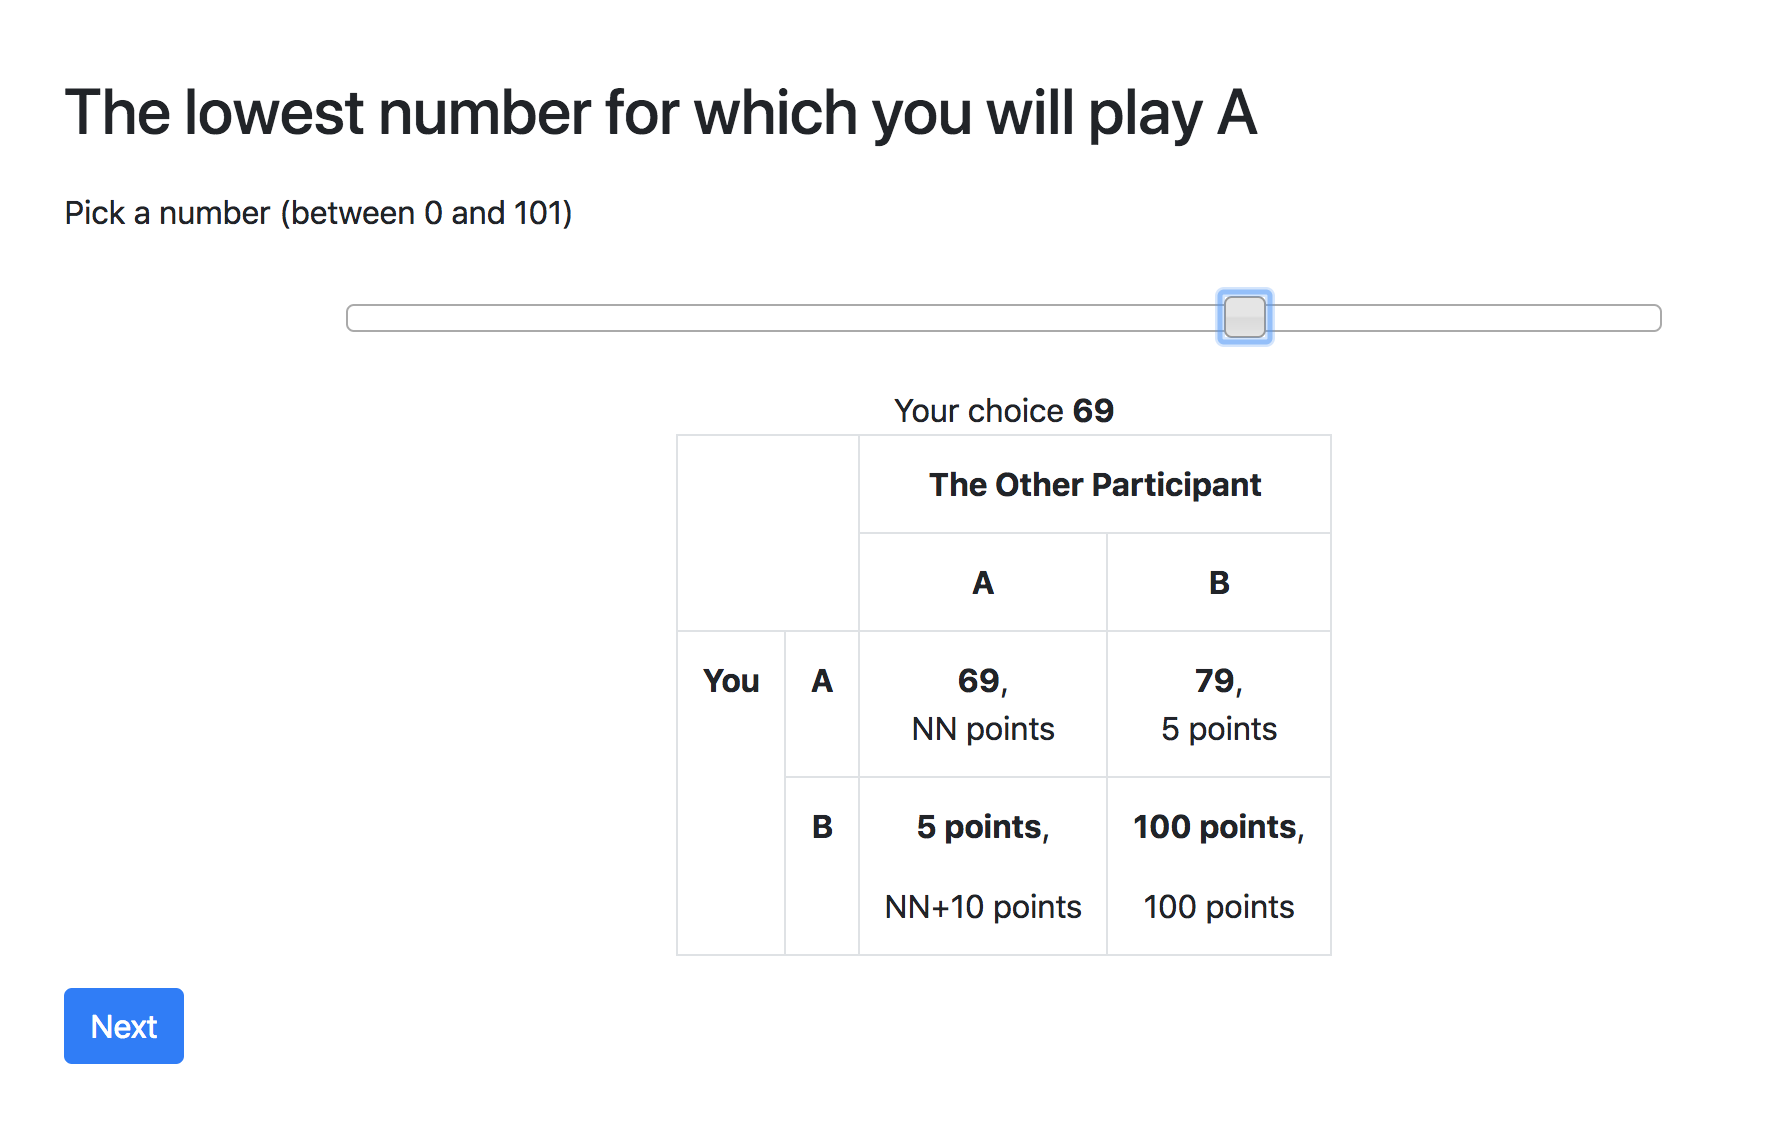
\includegraphics[scale=0.3]{cutoffen.png}%
\caption{User-Interface cutoff decision} 
\label{fig:ui}
\end{figure}
\end{center}
In each silo, the game started with five solo practice rounds. The counterparty is a robot that plays the NE prediction. The subject's task is to pick the minimum number of $x$ in the interval $[0,101]$ for which she will play $H$ (labelled $A$ in the experiment). That is, we directly ask the subject to select a cutoff strategy without having knowledge of her value of $x$ as well as the counterparty's value. The user-interface designed in oTree (Chen, et al., 2016) is depicted in Figure \ref{fig:ui}. Specifically, in order to select a cutoff value, the participant uses the mouse to move the slider. Then, to confirm her choice, the participant clicks on the button ``Next." Thus, a subject who wants to always play $D$ ($H$)  moves the slider to the extreme right (left). The user-interface also presents the updated payoff matrix with the cutoff selection. In the payoff matrix, the unknown value of $x$ for the counterparty is depicted as $NN$.

Following the five practice rounds, subjects played the 11 paid rounds. Each participant meets another participant once and only once (perfect stranger matching).\footnote{Alternatively, one can employ a mean matching protocol as in Hawk-Dove population games (Oprea, et al., 2011 and Benndorf, et al. 2016) for the simultaneous move game. A mean matching in the endogenous timing game brings technical difficulties in its implementation.} Subjects in all treatments make the cutoff choice simultaneously. Subjects do no not know their counterparty's gender. The next steps after choosing the cutoff value vary according to treatment. We summarize the different steps in Table \ref{table:time}. 

\begin{table}[ht]
\begin{center}
\begin{tabular}{l|m{2.4cm}|m{3.5cm}|m{4cm}}
  Step & CGO & CGS & CGE\\
  \hline 
I & Cutoff & Cutoff & Cutoff \\
\hline
II& $x_i$ is revealed; H if $\mtext{cutoff}\leq x_i$ & $x_i$ is revealed; H if $\mtext{cutoff}\leq x_i$ for 1st mover (randomly chosen)
& $x_i$ is revealed; choose $t=\{1,2\}$ with action commitment defined according to $\mtext{cutoff}$\\
\hline
III & - & 2nd mover picks \textbf{s} & 2nd mover ($t=2$) picks \textbf{s} if other chose $t=1$. Otherwise, the game is a oneshot.

\end{tabular}
\end{center}
\caption{Timeline for each treatment}
\label{table:time}
\end{table}

In the CGO game, the value of $x_i$ is revealed to player $i$. The subject plays $H$ if her cutoff choice is smaller than or equal to $x_i$. She plays $D$ otherwise. Given the actions $H$ or $D$ for both players, payoffs are computed according to the payoff matrix in equation (\ref{t:payoff}). 

In the $CGS$ game, a first mover is selected randomly after all subjects completed the cutoff choice. This procedure helps us to collect cutoff information for all subjects independently if they are first or second movers, and allows us to have a fairly balance number of silos across treatments. Here, it is also important to emphasize that all subjects know that their cutoff decisions are binding (relaxed) if they are first (second) movers. The second mover picks an action $s\in\{H,D\}$ conditional on the first mover's action. That is, the second mover does not face the same payoff matrix presented to the subjects in the $CGO $ game. Instead, the payoff matrix in the $CGS$ game only reflects the action selected by the first mover. 

In the $CGE$ game, subjects commit to the action mapped from the cutoff choice. They then decide when to play the game. If both players select the same period of play, then the game becomes a one shot game. If one player picks the first period while the other player picks the second period, then we are in the $CGS$ game, where the cutoff choice for the second mover is relaxed. The second mover makes a decision knowing what the first mover played. 

At the end of each round, for all treatments, we provide feedback regarding player choices as well as individual payoff information. After the 11 rounds were completed, the total points were converted to COL at the exchange rate of COL 20 per point. Earnings, including a show-up fee of COL 10,000 (\$ 3.3), were paid in cash. On average, players earned 792.8 points (\$ 5.2) for a session that lasted under 45 minutes. Table \ref{session} presents the average profit as well as other relevant information per treatment. 

\begin{table}[ht]
\centering
\caption{Sessions overview }
\hline
\begin{tabular}{lcccc}
  Treatment & Groups & Subjects per group & \% of women & Profit (mean, points)\\
  \hline  
  CGO & 6 & 12 & 51 & 701.6 \\
  CGS & 6 & 12 & 51 & 856.3 \\
  CGE & 6 & 12 & 47 & 820.7 \\
\hline
Total & 18 & 216 &  50 (mean) & 792.8 (mean)\\
\end{tabular}

\label{session}
\end{table}

\begin{center}
\begin{figure}[ht]
\centering{}%
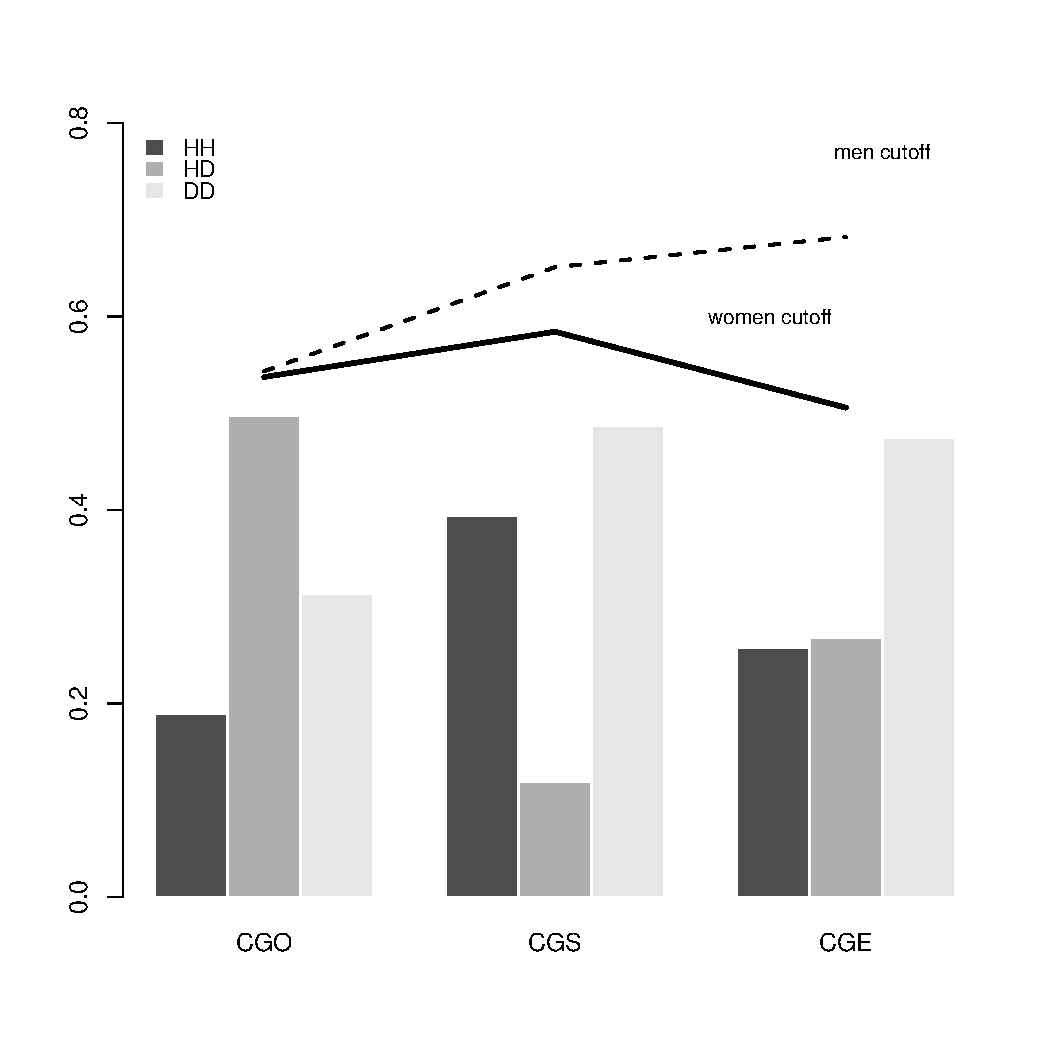
\includegraphics[scale=0.5]{jointcut.pdf}%
\caption{Cutoff strategy and cell relative frequencies across treatments (pooled data)} 
\label{fig:cutpooled}
\end{figure}
\par\end{center}


\section{Results}
\label{sec:results}

We begin by presenting in Figure \ref{fig:cutpooled} pooled data across all three treatments.\footnote{The data collected from the experimental sessions, as well as the data analysis included in this paper, can be found at \url{https://github.com/rabsjp/hdseq}.} In the $CGO$ treatment the mean cutoff is around 50 percent, which is consistent with previous experimental work (e.g. see Evdokimov and Garfagnini, 2018). We count the frequency of each outcome ($HH$, $HD (=DH)$ and $DD$) and determine that for the baseline $CGO$ game (i) the $DD$ outcome is around 30 percent, and (ii) the off-diagonal cells appear most often, at around 50 percent. The outcomes for both the $CGS$ and $CGE$ treatments are quite different from the $CGO$ outcomes. Subjects in the $CGS$ game increase the mean cutoff value to around 60 percent, and men appear to increase the cutoff more relative to women. The sequential order of play helps achieve greater coordination with respect to the $DD$ and $HH$ outcomes, which occur around 50 percent and 40 percent of the time, respectively. 

\begin{center}
\begin{figure}[ht]
\centering{}%
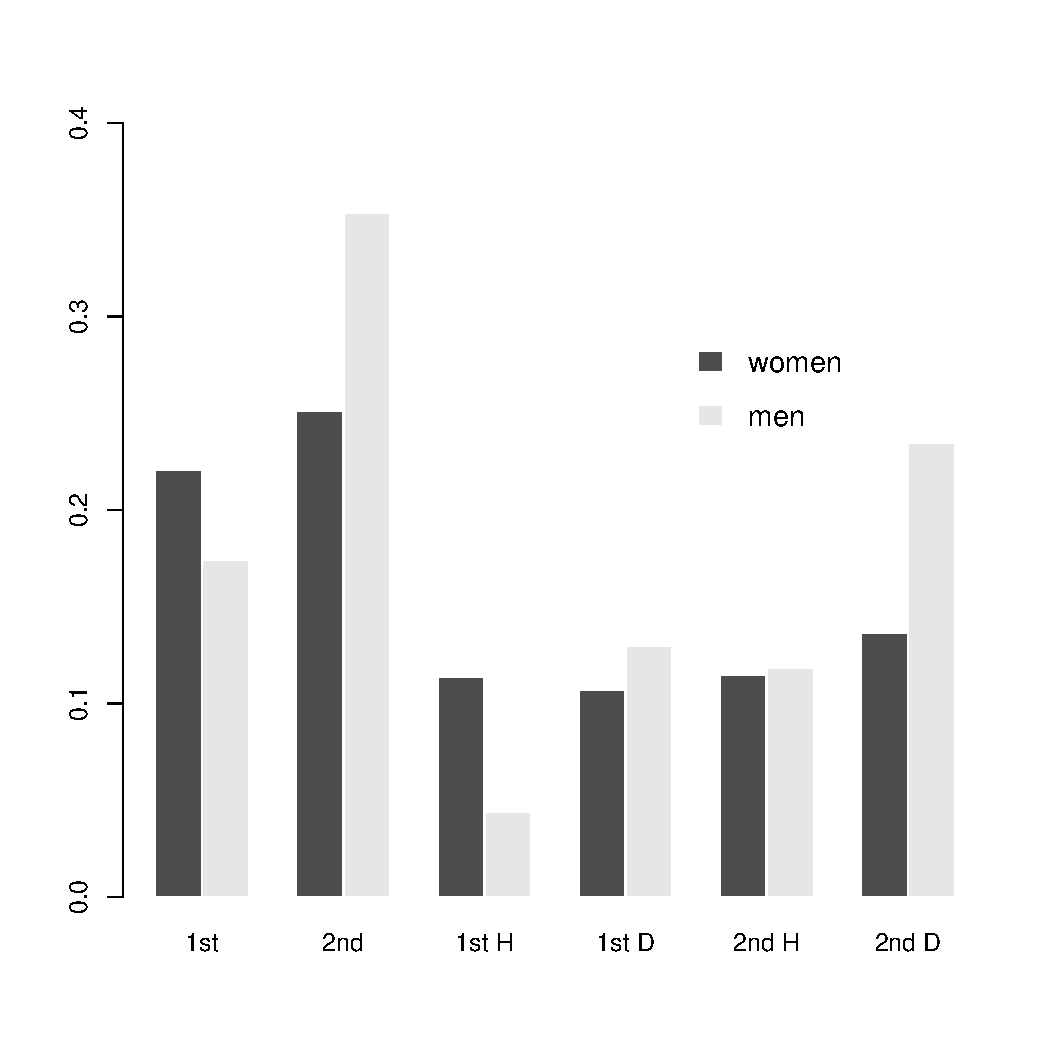
\includegraphics[scale=0.5]{countgendermoveplay.pdf}%
\caption{Strategy and order of play by gender (CGE)} 
\label{fig:cgepooled}
\end{figure}
\end{center}

The $CGE$ game presents a similar level of coordination with respect to the $DD$ outcome as the $CGS$ game. The mean cutoff by gender, however, is quite different. The cutoff strategy chosen by women in the $CGE$ game is similar to their strategy in the $CGO$ game. The men, on the other hand, increase their cutoff strategy, relative to the $CGS$ game. Next, we analyze gender differences in the $CGE$ game according to strategy and order of play. The first two columns of Figure \ref{fig:cgepooled} present the time period $t\in\{1,2\}$ preference by gender. We can clearly see that men prefer to move second while women's choices are evenly distributed across both periods. Furthermore, men appear to play $D$ more often than women across both periods, which is consistent with the different cutoff strategies illustrated in Figure \ref{fig:cutpooled}.

\begin{table}[!t]
\centering\caption{Frequency (\%) by action and encounter type ($CGE$)}

\begin{tabular}{lccc}
\hline
 & One-shot 1st period & One-shot 2nd period  & Sequential\\
  \hline
  $HH$ &  2.27 & 5.56 & 17.93 \\
  $HD$ & 5.81 & 15.91 & 5.05 \\
  $DD$& 5.30 & 12.88 & 29.29 \\
  \hline
Total & 13.38 & 34.35 & 52.27\\
\end{tabular}

\label{tab(CGE)}
\end{table}

Table \ref{tab(CGE)} details the frequency of the outcomes, $HH$, $HD(\equiv DH)$ and $DD$, tabulated according to the types of encounters possible in the $CGE$ environment. That is, we summarize the frequency for each cell in a one-shot game played in the first period, one-shot game played in the second period, and a sequential order of play when subjects have different time preferences. About 52 percent of encounters occur sequentially. Of those, 56 percent lead to the $DD$ outcome. Most of the simultaneous encounters happen in the second period, and 41 percent of them lead to $DD$ outcome.  \\

\begin{center}
\begin{figure}[ht]
\centering{}%
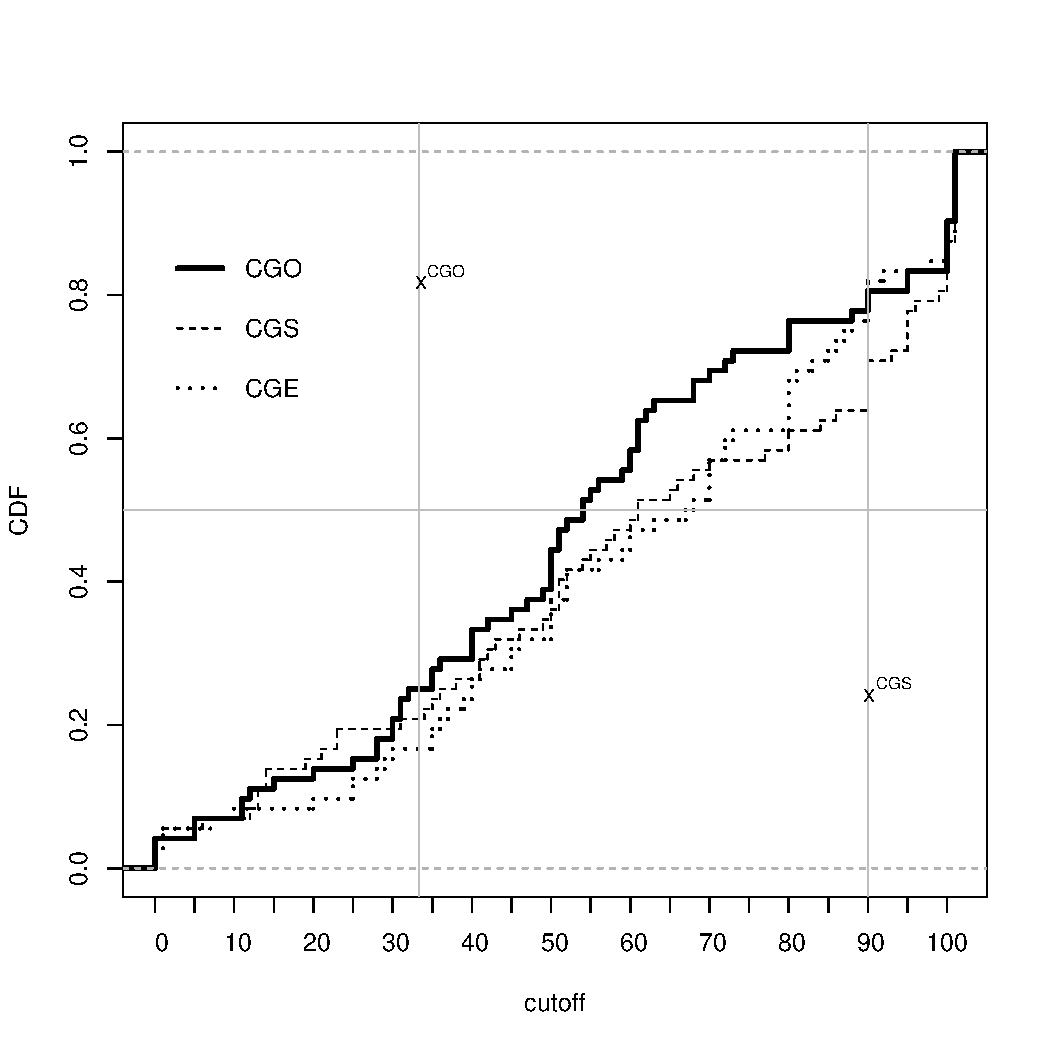
\includegraphics[scale=0.5]{cdfcutoff.pdf}%
\caption{CDF of cutoff strategies (subject data) \\ } 
\label{fig:allcutoff}
\floatfoot{\footnotesize{\textit{Note: $x^{CGO}$ ($x^{CGS}$) is the predicted cutoff in the CGO (CGS) game.}}}
\end{figure}
\par\end{center}

\noindent \textbf{Result 1}
\textit{The median cutoff strategy in the $CGO$ game is 50 percent.}

We first take a conservative approach to testing our predictions. We compute the median cutoff chosen by each subject in rounds 6 through 11. Figure  \ref{fig:allcutoff} presents CDF by treatment. In the $CGO$ game, we can see that the median value is 50 percent, and that the distribution is fairly uniform, with some qualifications. About 20 percent of subjects pick the highest cutoff, which indicates that they strongly prefer to play $D$. Furthermore, we observe no significant mass centered around 33 percent, which is the NE prediction. In fact, the Kolmogorov-Smirnov (KS) test strongly rejects the hypothesis that cutoff strategy in the $CGO$ game is equal to or below the NE prediction (the p-value is 2.2e-16).

To control for group effects we also perform panel regressions (OLS), presented in Table \ref{table:olscgs}, which confirm the results from our non-parametric analysis using all eleven periods. We evaluate three alternative dependent variables-- cutoff choice, profit and play of $D$--  on different regressors, including: variable $CGS$ which takes on the value of one for the $CGS$ treatment and zero otherwise; the trend variable $Period$ which controls for learning throughout the session; the interaction between the trend and the treatment $Period \times CGS$; the gender variable $Men$ which takes on the value of one when the subject is a man and zero otherwise; and the interaction effect between gender and treatment $Men \times CGS$. The mean cutoff choice in the $CGO$ treatment (specification I) is about 50 which is above the NE prediction of 33. Players get an average profit of 62 points (specification II).\footnote{The variable $Period$ is analyzed at the mean of six, when it is statistically significant.} Players in the $CGO$ treatment decrease their cutoff choice in later periods as suggested by the negative sign of the trend, which weakly increases profit (the sign of the trend is positive in specification II, though not statistically significant). The extremely low $R^2$ in the regressions is due to the high heterogeneity observed in the cutoff choices (and therefore profit) common in these games (e.g. see Duffy and Ochs, 2012).\\

\noindent \textbf{Result 2}
\textit{In the $CGS$ game, players increase the median cutoff to 66 percent.}

The CDF for the $CGS$ game first-order stochastically dominates the CDF for $CGO$ game (the p-value of a Kolmogorov-Smirnov test for which the null states that $\hat{x}_{_{CGO}} \geq \hat{x}_{_{CGS}}$ is 0.006). The mass in the $CGS$ game approaches the predicted NE of 90 percent, thought it still falls short. The median cutoff strategy is 66 percent. Similar to the $CGO$ environment, some players in the $CGS$ game also select either extremely high or extremely low cutoff values. Overall, the majority of players in the $CGS$ game select a higher threshold relative to the $CGO$ game, thus improving social welfare.\footnote{If we include all periods in KS test, we obtain a p-value of 0.19. Therefore, we fail to reject that $CGO$ and $CGS$ distributions are equal. The significance (at five percent) of the results appears from periods 3 to 11. Our sample includes periods 6 to 11 to account for learning.}

Table \ref{table:olscgs} compares the choices (specification I) and profit (specification II) in $CGO$ and $CGS$ treatments using panel regressions (OLS). The mean cutoff choice in the $CGO$ treatment is lower than in the $CGS$ treatment by about 9 points. The average profit for players in the $CGS$ treatment is higher by about 15 points. The interaction between the trend variable and $CGS$ shows that players in the $CGS$ treatment increase their cutoff strategy as the game progresses, contrary to the behavior observed in the $CGO$ treatment. Thus, our results suggest that strategies are influenced by the environment, even though on average we observe similar frequencies of $D$ play (specification V, Table \ref{table:olscgs}). The lack of statistical significance for the treatment variable in specification V can be explained by the small number of observations we have to account for meaningful difference of play given that cutoff choices vary by approximately 10 percent across treatments, and the choices are quite dispersed across subjects.\\ 

\begin{table}[ht]
\centering
\caption{Panel Regressions (OLS)}
\footnotesize
\begin{tabular}{lcc|cc|cc}
  \hline
  &\multicolumn{2}{c|}{CGO vs CGS} &\multicolumn{2}{c|}{CGE vs CGS} & CGO vs CGS& CGE vs CGS\\
  & (I) & (II) & (III) & (IV) & (V) & (VI)\\
&  cutoff & profit & cutoff & profit & play D & play D \\
    \hline
Intercept & $56.04^{^{***}}$ &  $ 61.86^{^{***}}$ & $47.88^{^{***}}$ &  $66.43^{^{***}}$ & $0.57^{^{***}}$& $0.52^{^{***}}$\\
& (5.09) & (4.76) & (3.21) & (4.45) & (0.04) & (0.05)\\
Period & $-0.54^{^{**}}$ & $0.26$ & $1.02^{^{**}}$ & $1.11^{^{***}}$ & -- & -- \\
& (0.17)&  (0.47) & (0.33)&  (0.24) & & \\
CGS & $-1.24$ &  $14.95^{^{**}}$ & $  2.74$ &  $9.34$ &  $-0.05$ & 0.00\\
& (5.60) & (5.95) & (3.50) & (5.96) & (0.06) & (0.06)\\
Period $\times$ CGS & $1.50^{^{**}}$& $-0.15$ & $-0.07$&$-1.00^{^{*}}$ & -- & -- \\
& (0.53) & (0.69) & (0.53) & (0.55) & &  \\
Men & $3.67$ &  $0.69$ & $12.27^{^{***}}$ &  $2.85^{^{*}}$ & $-0.02$ & $0.18^{^{***}}$ \\
& (3.57) & (1.61) & (4.42) & (1.75) & (0.04) & (0.05)\\
Men $\times$ CGS & --& --& --& -- & 0.08 & $-0.12^{^{*}}$\\
& & & & & (0.08) & (0.06)\\
\hline
N & 1,584 & 1,584 & 1,584 & 1,584 & 1,584  & 1,584 \\ 
$R^2$ & 0.02 & 0.04 & 0.04 & 0.01 & 0.00 & 0.02\\
\hline
\hline
 \multicolumn{7}{p{.9\textwidth}}{\scriptsize{The dependent variable in (I) and (III) is the cutoff choice. In specifications (II) and (IV) the dependent variable is the profit earned. Standard errors are in parenthesis, clustered at the group level and are computed via bootstrapping. Random effects are included at the subject level. }}\\ 
 \multicolumn{3}{p{0.4\textwidth}}{\scriptsize{ $^{^{***}}p\leq.01$,
    $^{^{**}}p\leq.05$, $^{^{*}}p\leq.1$}} \\
\end{tabular}
\label{table:olscgs}
\end{table}

\noindent \textbf{Result 3}
\textit{In the $CGE$ game the median cutoff strategy is 70 percent.}

While roughly 25 percent of players select a low cutoff strategy similar to the one in the $CGO$ game, the majority of players select a cutoff value such that $\hat{x}_{_{CGE}}> \hat{x}_{_{CGO}}$. There is also a sizable mass (35 percent) of players who select a cutoff strategy with values above the predicted NE of 90 in the $CGS$ game. The overall distribution of cutoff strategies in the $CGE$ game is quite similar to the one in the $CGS$ game. We fail to reject the hypothesis that the two cutoff strategies come from the same distribution (KS test p-value of 0.77).

The regressions (see Table \ref{table:olscgs}) confirm that cutoff strategy (specification III) and play of $D$ (specification VI) are similar across the $CGE$ and $CGS$ treatment. In terms of profit (specification IV), players in the $CGS$ perform slightly worse (about 6 point difference).\\

\noindent \textbf{Result 4}
\textit{The $DD$ outcome appears more often in $CGS$ and $CGE$ environments.}

We compute the frequency with which $DD$ appears in each of the groups (of twelve people). Table \ref{table:dd} presents the sorted data and the mean per treatment. $DD$ occurs less often in the $CGO$ environment across all six independent groups. $CGS$ and $CGE$ do not exhibit low $DD$ frequency ($<$ 30 percent), which appear in two-thirds of the $CGO$ groups. More formally, non-parametric tests reject the hypothesis that the frequency of $DD$ in the $CGO$ environment is greater than or equal to either the frequency of $DD$ in $CGS$ (KS p-value of 0.069 and Wilcoxon p-value of 0.018) or $CGE$ (KS p-value of 0.069 and Wilcoxon p-value of 0.015) environment. Additionally, we fail to reject the hypothesis that $CGS$ and $CGE$ come from the same distribution (p-value of a Wilcoxon two-sided test is 1.0).\footnote{We omit panel regressions when analyzing the joint frequency given that the non-parametric tests are at the group level which strictly satisfies the independence assumption across observations. Using all periods does not change the conclusions of our tests. When comparing $CGO$ vs $CGS$, the KS test p-value is 0.016 and Wilcoxon test p-value is 0.020. When comparing $CGO$ vs $CGE$, the KS test p-value is 0.069 and Wilcoxon test p-value is 0.063. }\\

\begin{table}[!t]
\centering
\caption{Frequency (percentage) of cell $DD$ played in groups }
\begin{tabular}{lccccccc}
\hline
Treatment & Group 1 & G2  & G3 & G4 & G5 & G6 & Mean\\
  \hline
  CGO &  19.44 & 19.44&  27.78 & 27.78 & 36.11 & 52.78 & 30.56 \\
  CGS & 30.56 & 47.22&  50.00 & 52.78 & 55.56 & 61.11 & 49.53\\
  GGE & 33.44 & 38.49 & 44.44 & 58.55 & 63.89 & 69.44 & 51.39 \\
  \hline

\end{tabular}

\label{table:dd}
\end{table}

\noindent \textbf{Result 5}
\textit{Gender differences appear only in the $CGE$ game. Men significantly increase their cutoff value, improving the frequency with which $D$ is selected, while women revert to a strategy similar to the one in the $CGO$ game.}

We next analyze the cutoff strategy across gender. Figure \ref{fig:cdfgender1} presents the CDF of the cutoff strategy by gender in the $CGO$ game (left panel) and the $CGS$  game (right panel). We find no difference in strategy in the $CGO$ game (KS test p-value 0.52). In the $CGS$ game, we observe a larger mass of men with a cutoff strategy that is greater than the predicted NE (90). The rest of the distribution looks quite similar across gender. In fact, we fail to reject the hypothesis that the cutoff distributions are equal in the $CGS$ game (KS p-value of 0.54). It is important to note that in the $CGS$ game, conditional on observing $D$ in the first period, we do not observe any gender difference among the second mover responses. There are about 10 percent of women and men who follow $D$ with an $H$ choice, which is consistent with theory.

\begin{center}
\begin{figure}[ht]
\centering{}%
\begin{minipage}[t]{0.45\columnwidth}%
\subfloat{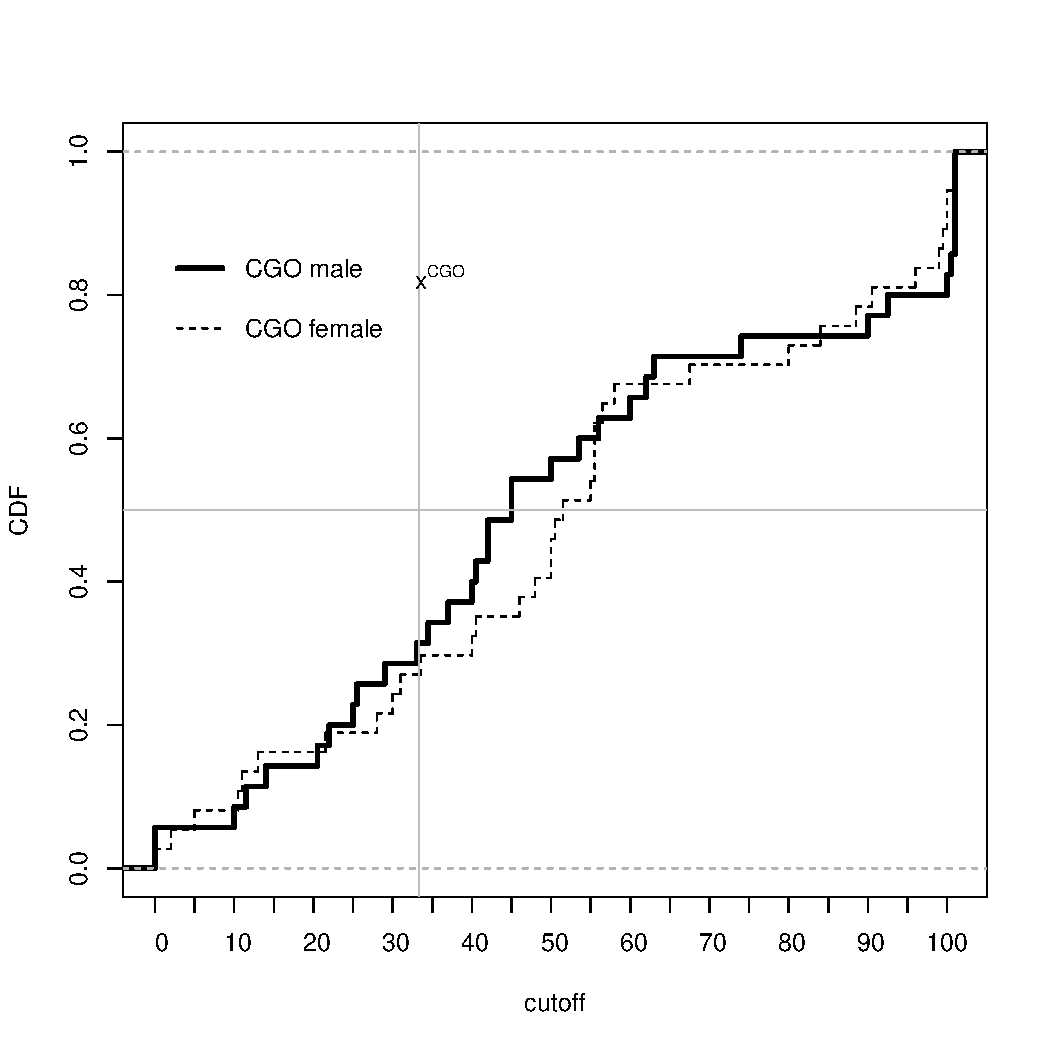
\includegraphics[scale=0.4]{cdfcutoffgender_o.pdf}}%
\end{minipage}%
\begin{minipage}[t]{0.45\columnwidth}%
\subfloat{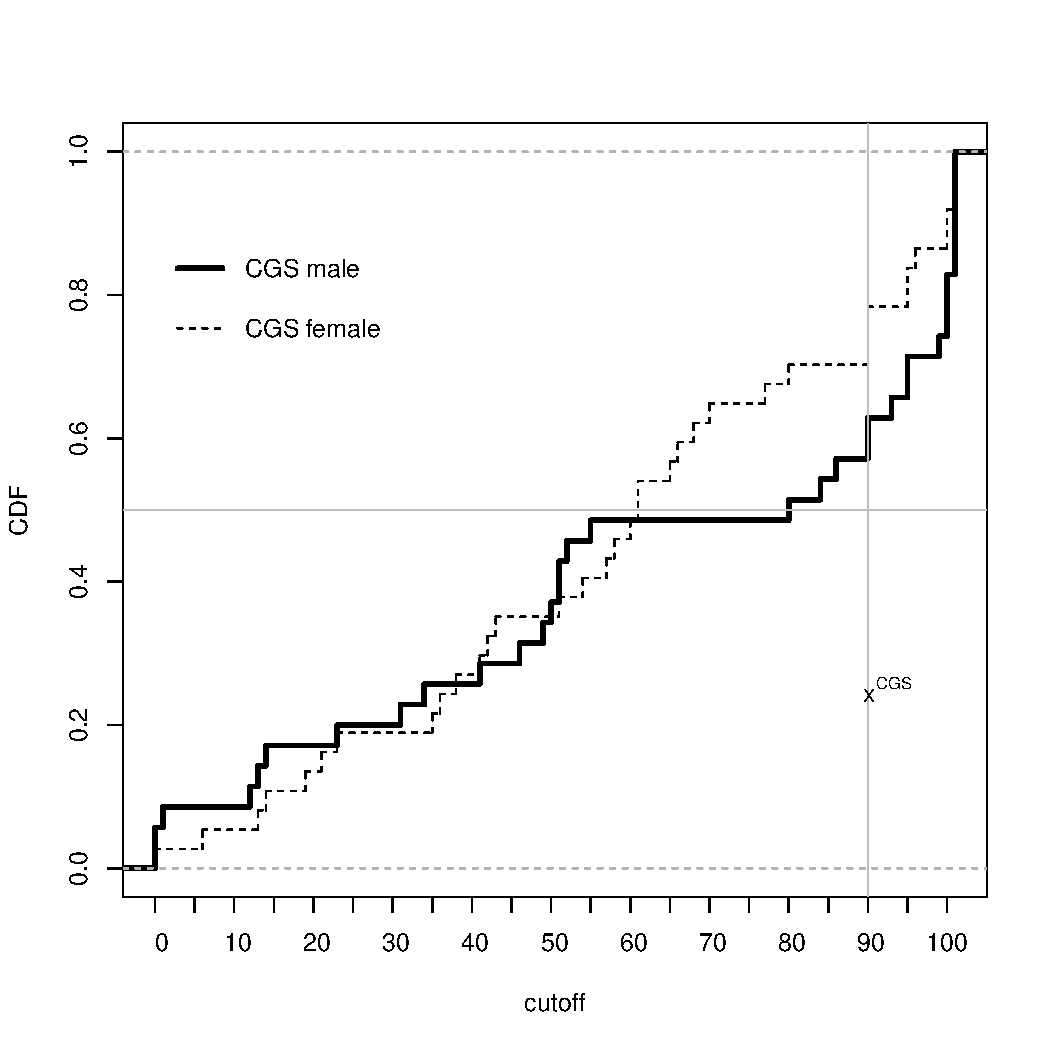
\includegraphics[scale=0.4]{cdfcutoffgender_s.pdf}}%
\end{minipage} 
%\captionsetup{font=large}
\caption{CDF of cutoff strategy choices in CGO (left) and CGS (right), by gender \\\footnotesize{\textit{Note: $x^{CGO}$ ($x^{CGS}$) is the predicted cutoff in the $CGO$ ($CGS$) game.}} }
\label{fig:cdfgender1}\end{figure}
\par\end{center}
%0.06258w
%0.07457ks
However, important differences emerge under endogenous timing. The cutoff strategy choices by men first order stochastically dominate the cutoff strategy choices by women, which we depict in the left panel of Figure \ref{fig:cdfgender2}. We reject the null hypothesis which states that men choose a cutoff strategy that is equal to or smaller than the one chosen by women, with a p-value of 0.001 for Wilcoxon and 0.006 for KS.\footnote{Using all periods, we also confirm the separation between cutoffs. The p-values are 0.06 for Wilcoxon and 0.01 for KS.} The cutoff strategy distribution for women in the $CGE$ game resembles the one observed in $CGO$ game. The cutoff strategy distribution for men shifts significantly to the right, such that the median value is closer to the one observed in the $CGS$ game. The mass around the high cutoff strategy choices ($>$90) in both $CGS$ and $CGE$ is about 40 percent for men. This is quite different than the behavior observed in $CGO$, where the mass is about 20 percent. 

The high cutoff values chosen by men translates to a higher frequency of $D$ play as shown in the right panel of Figure \ref{fig:cdfgender2}. Corroborating our earlier conclusion, the frequency of $D$ choices across gender shows neither statistical nor economic differences across $CGO$ and $CGS$ games. We find a difference in $D$ play across gender only in the $CGE$ game. Specifically, in this environment the results show that men play $D$ at a rate of 20 percentage points higher than women. 

\begin{center}
\begin{figure}[ht]
\centering{}%
\begin{minipage}[t]{0.45\columnwidth}%
\subfloat{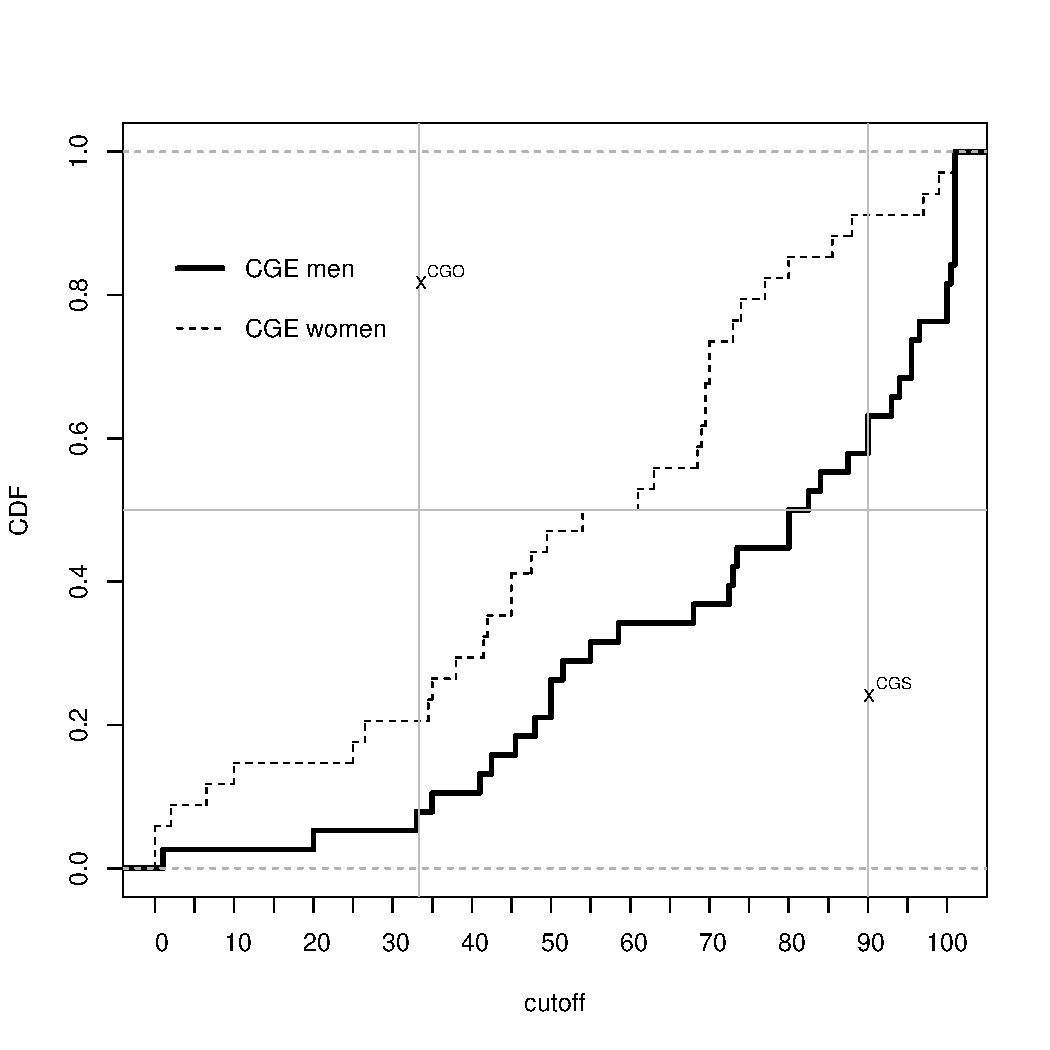
\includegraphics[scale=0.4]{cdfcutoffgender_e1.pdf}}%
\end{minipage}%
\begin{minipage}[t]{0.45\columnwidth}%
\subfloat{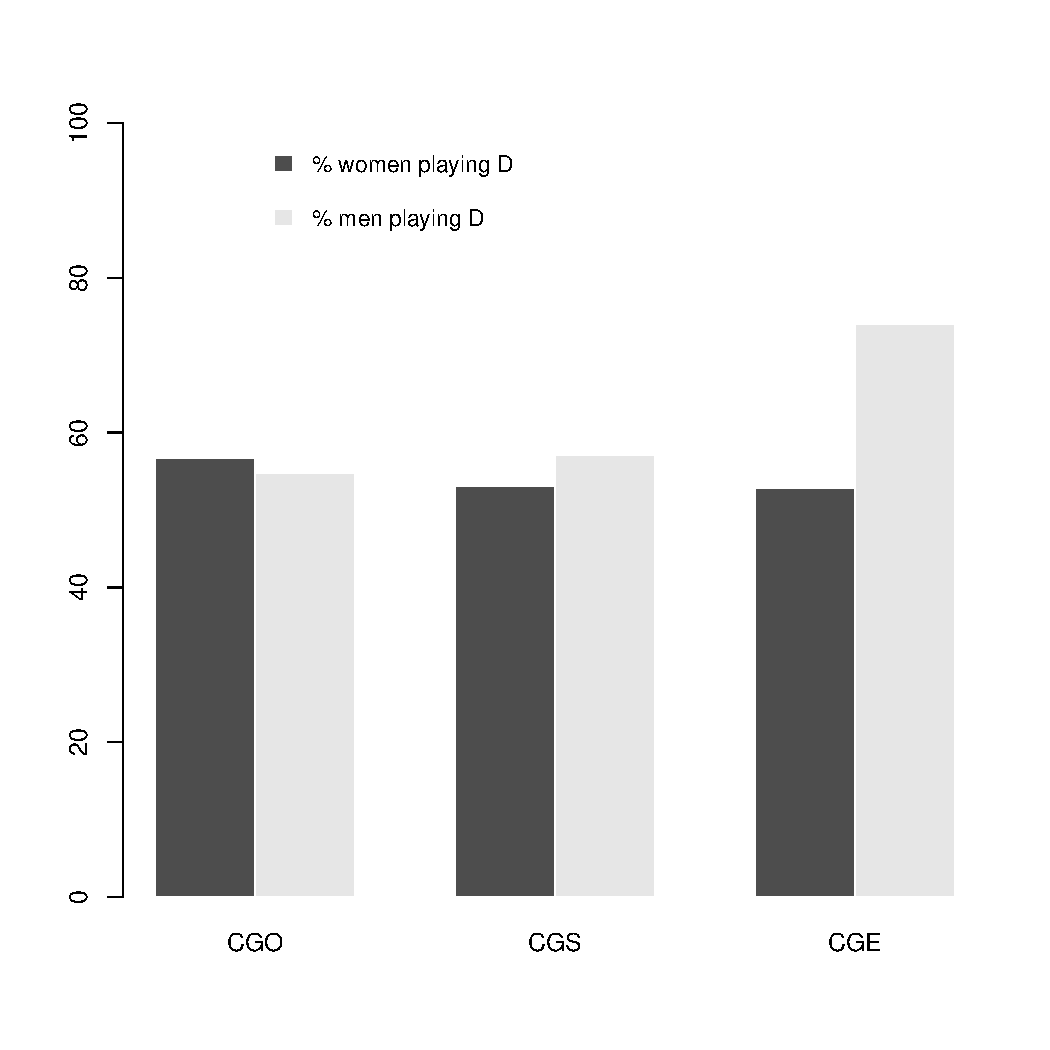
\includegraphics[scale=0.4]{genderplay1.pdf}}%
\end{minipage} 
%\captionsetup{font=large}
\caption{CDF of cutoff strategies in $CGE$ (left panel) and $D$ play (right panel) by gender\\ \footnotesize{\textit{Note: $x^{CGO}$ ($x^{CGS}$) is the predicted cutoff in the $CGO$ ($CGS$) game.}}}
\label{fig:cdfgender2}\end{figure}
\par\end{center}

\begin{center}
\begin{figure}[ht]
\centering{}%
\begin{minipage}[t]{0.45\columnwidth}%
\subfloat{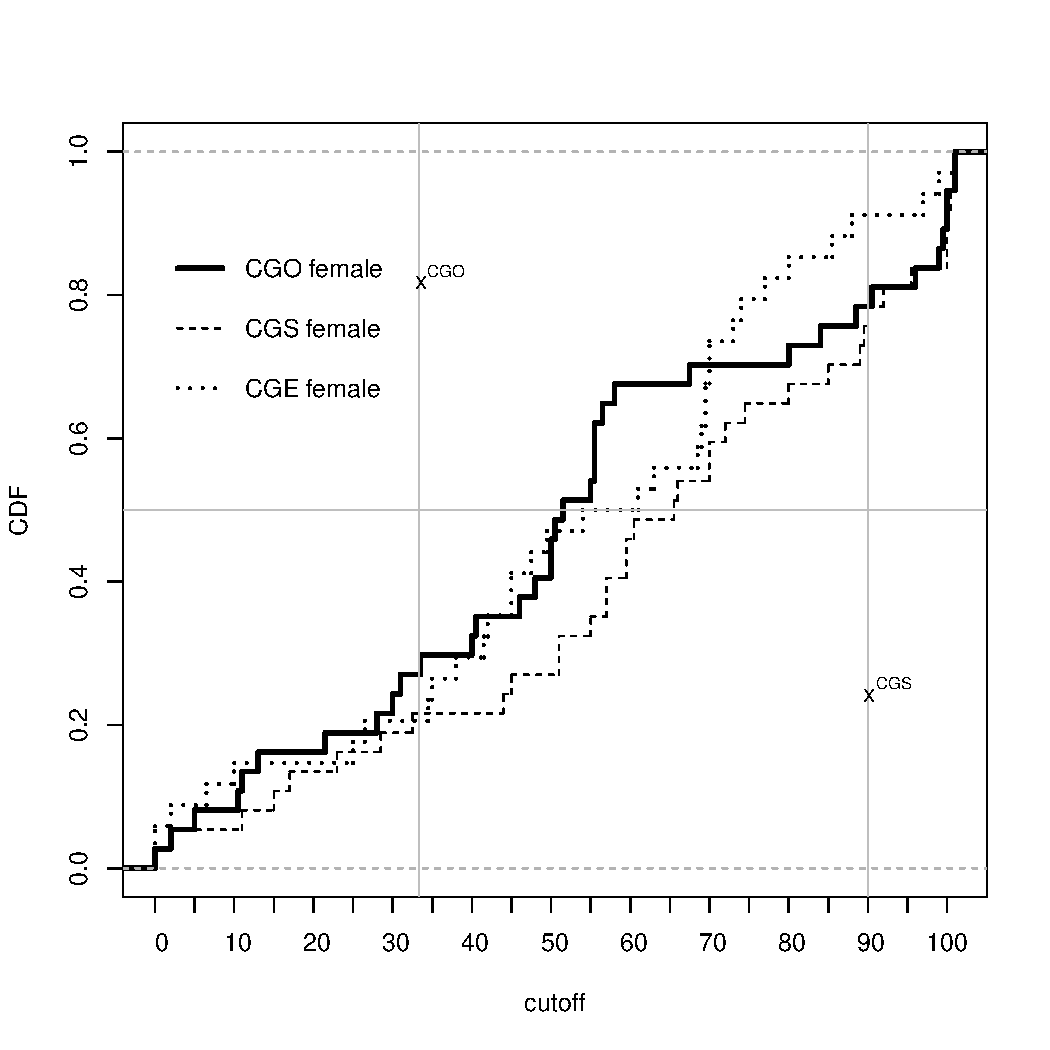
\includegraphics[scale=0.4]{cdfcutoffgender_female.pdf}}%
\end{minipage}%
\begin{minipage}[t]{0.45\columnwidth}%
\subfloat{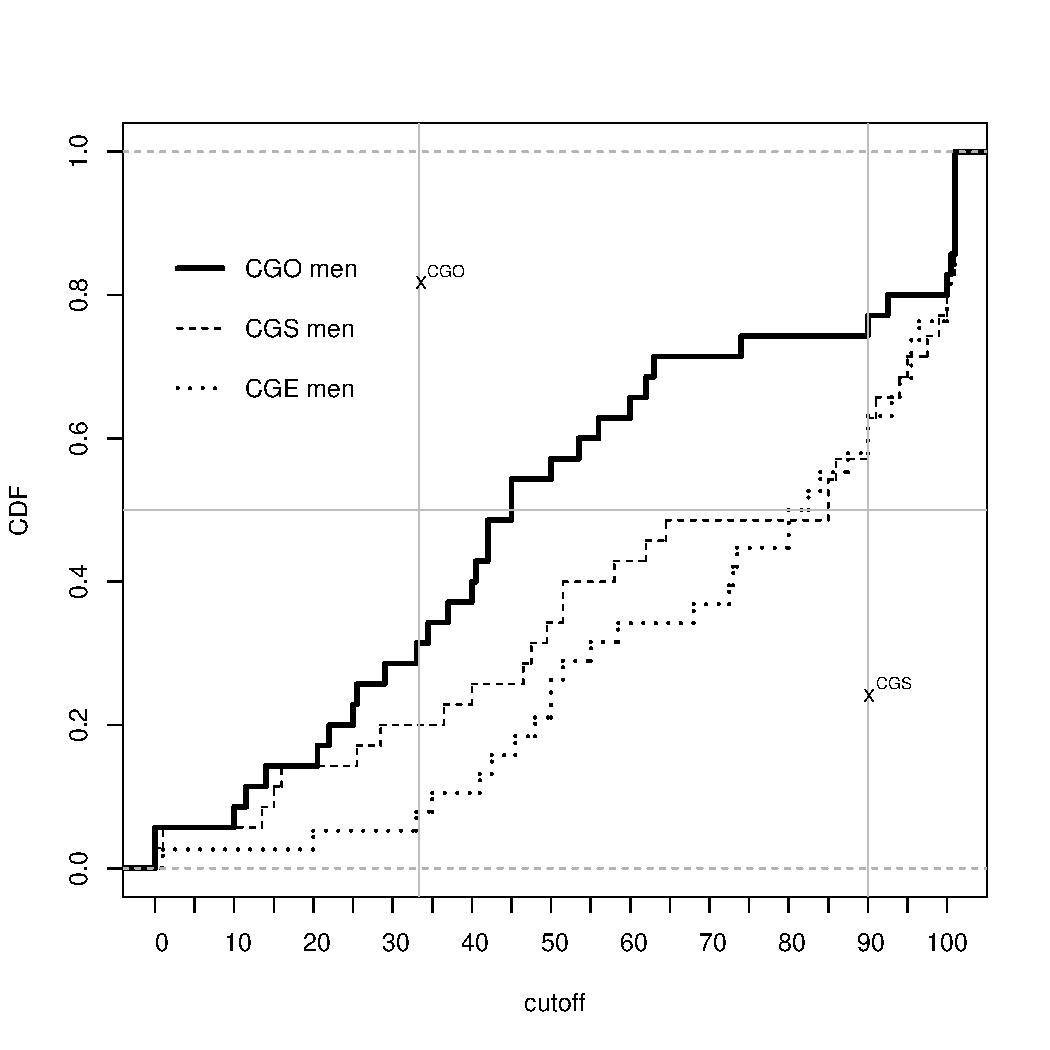
\includegraphics[scale=0.4]{cdfcutoffgender_male.pdf}}%
\end{minipage} 
%\captionsetup{font=large}
\caption{CDF of cutoff strategies for women (left) and men (right) across treatments\\\footnotesize{\textit{Note: $x^{CGO}$ ($x^{CGS}$) is the predicted cutoff in the $CGO$ ($CGS$) game.}}}
\label{fig:cdfall}\end{figure}
\par\end{center}

Table \ref{table:olscgs} also shows gender differences using panel (OLS) regressions. The variable $Men$ is significant only in the $CGE$ treatment. Men increase their cutoff relative to women by 12 points, which translates to slightly higher profits (about 3 points, at a 10 percent significance level) and higher frequency of $D$ (18 percentage points).\foonote{The payoff gain for men is also small (about 5) if we restrict the sample to the $CGE$ treatment only.}

\section{Discussion}
\label{sec:discuss}

In this paper, we find evidence of gender differences in strategic behavior under endogenous timing conflict game with strategic complements. Our design builds on the BS04 conflict game, which we present in a Hawk-Dove environment, and varies the timing and extent of commitment by players to an $H$ or $D$ action. Early commitment to $D$ is risky because a player can lose 95 percent of the (Pareto) payout if the counterparty plays $H$. Early commitment to $H$ can lead to a payoff of either $x$ or $x+10$, when the counterparty chooses either $H$ or $D$, respectively.  Note that since  $x$ is randomly drawn from a uniform distribution with support $[0,100]$, a player is uncertain of how hawkish the counterparty may be. The experimental results suggest that men are less risk averse to selecting $D$ relative to women in the presence of strategic uncertainty. The gender difference is quite remarkable compared to our two other treatments, $CGO$ and $CGS$, where strategic uncertainty, which arises due to lack of knowledge about counterparty type/action and the order of player, is removed.

The conflict game we study has different applications, as many contest games do.\footnote{For an overview of recent theoretical models of war and conflict as well as the empirical literature using laboratory and field data, please refer to Kimbrough et al. (2017).}  For example, our game can be interpreted as a bank-run model or a conflict featuring sanctions and/or tariffs, and any other game featuring strategic complementarity. In the bank-run analogy, agents have the option to withdraw ($H$) or not ($D$), and are uncertain about the  liquidity cost (or type of the counterparty, which determines the action). To the best of our knowledge, Kiss et al. (2014) and Dijk (2017) are the only bank-run experiments to study gender.\footnote{On the theory side, there is an established tradition of modeling bank runs or attacks using techniques from global games. See Goldstein and Pauzner (2004, 2005), Morris and Shin (2003, 2004a, 2004b), Guimaraes and Morris (2007), Rochet and Vives (2004), among others.} Kiss et al. do not find significant differences on withdrawing rates across gender, which is similar to what we find in our sequential game.  Dijk reports that women are more likely to withdraw as fear increases. Our results would then indicate that under risky commitment, withdrawing rates should be higher for women than for men.

Considering the different conclusions in literature on gender differences in risk attitudes, and the role of social norms, future field or experimental work can complement the findings documented in this paper.

\section{Acknowledgements}
We are grateful for the comments received from Lata Gangadharan, Dan Friedman, Tomas Sj\"ostr\"om, Dann Arce, Nisvan Erkal, Diego Aycinena, Kyung Hwan Baik, Tom Wilkening, Maria Recalde, Tim Cason, John Duffy, David Gill, Jin Yeub Kim, Roman Sheremeta, and seminar participants at the 2018 Southern Economic Association meetings, the 2018 Stony Brook Game Theory Festival, the 2018 New England Experimental Economics Workshop, the 2018 Maine Economics Conference, the University of Melbourne and the University San Francisco de Quito. This research was supported by funds granted by Colby College. This project was approved by the IRB at Colby College and Universidad del Rosario.

\newpage
\begin{thebibliography}{10}

\bibitem{} Andreoni, J., 1998. Toward a theory of charitable fund-raising. \textit{Journal of Political Economy,} 106(6), pp.1186-1213.

\bibitem{} Azmat, G., Calsamiglia, C. and Iriberri, N., 2016. Gender differences in response to big stakes. \textit{Journal of the European Economic Association,} 14(6), pp.1372-1400.

\bibitem{} Babcock, L., Recalde, M.P., Vesterlund, L. and Weingart, L., 2017. Gender differences in accepting and receiving requests for tasks with low promotability. \textit{American Economic Review,} 107(3), pp.714-47.

\bibitem{} Baik, K.H. and Shogren, J.F., 1992. Strategic behavior in contests: comment. \textit{The American Economic Review,} 82(1), pp.359-362.

\bibitem{key-32}  Baliga, S. and Sj\"ostr\"om, T., 2004. Arms Races and Negotiations. \textit{Review of Economic Studies} 71, pp. 351-369.


%\bibitem{} Baliga, S, and Sj\"ostr\"om, T. 2009. Conflict Games with Payoff Uncertainty. Unpublished.


%\bibitem{} Baliga, S, and Sj\"ostr\"om, T. 2012 [A]. The Hobbesian Trap. In \textit{The Oxford Handbook of the Economics of Peace and Conflict}, edited by Michelle R. Garfinkel and Stergios Skaperdas. New York: Oxford University Press.

\bibitem{key-32}  Baliga, S. and Sj\"ostr\"om, T., 2012. The Strategy of Manipulating Conflict.\textit{American Economic Review} 102 (6), pp. 2897-2922.

\bibitem{key-32} Benndorf, V., Martinez-Martinez, I. and Normann, H.T., 2016. Equilibrium selection with coupled populations in hawk-dove games: Theory and experiment in continuous time. \textit{Journal of Economic Theory,} 165, pp.472-486.

\bibitem{key-32} Brindisi, F., \c{C}elen, B. and Hyndman, K., 2014. The effect of endogenous timing on coordination under asymmetric information: An experimental study. \textit{Games and Economic Behavior,} 86, pp.264-281.

\bibitem{} Cabrales, A., Nagel, R. and Armenter, R., 2007. Equilibrium selection through incomplete information in coordination games: an experimental study. \textit{Experimental Economics,} 10(3), pp.221-234.

\bibitem{} Carlsson, H. and Van Damme, E., 1993. Global games and equilibrium selection. \textit{Econometrica: Journal of the Econometric Society,} 61(5) pp.989-1018.

\bibitem{} Casari, M., Ham, J.C. and Kagel, J.H. 2007. Selection bias, demographic effects, and ability effects in common value auction experiments. \textit{American Economic Review,} 97, pp.1278-1304.

\bibitem{key-32} Chen, D.L., Schonger, M. and Wickens, C., 2016. oTree--An open-source platform for laboratory, online, and field experiments. \textit{Journal of Behavioral and Experimental Finance,} 9, pp.88-97.

\bibitem{key-32} Chen, Y., Katuscak, P. and Ozdenoren, E. 2013. Why can't a woman bid more like a man? \textit{Games and Economic Behavior,} 77, pp.181-213.

\bibitem{key-32} Chen, Z., Ong, D. and Sheremeta, R. 2015. The Gender Difference in the Value of Winning, \textit{Economics Letters,} 137, pp.226-229.

\bibitem{key-32}Dasgupta, A. 2007. Coordination and Delay in Global Games. \textit{Journal of Economic Theor,} 134(1), pp.195-225.

\bibitem{key-32} Di Girolamo, A. and Drouvelis, M., 2015. The role of gender composition and size of the group in a minimum effort game. \textit{Economics Letters,} 137, pp.168-170.

\bibitem{key-32} Dijk, O., 2017. Bank run psychology. \textit{Journal of Economic Behavior \& Organization,} 144, pp.87-96.

\bibitem{} Duffy, J. and Ochs, J., 2012. Equilibrium selection in static and dynamic entry games. \textit{Games and Economic Behavior,} 76(1), pp.97-116.

\bibitem{} Dufwenberg, M. and Gneezy, U., 2005. Gender \& coordination.In \textit{Experimental business research} (pp. 253-262). Springer, Boston, MA.

\bibitem{}Eaton, C.B., 2004. The elementary economics of social dilemmas. \textit{Canadian Journal of Economics/Revue canadienne d'\'{e}conomique,} 37(4), pp.805-829.

\bibitem{key-32}  Evdokimov, P. and Garfagnini, U., 2018. Third-party manipulation of conflict: an experiment. \textit{Experimental Economics,} 21(1), pp.27-49.

\bibitem{key-32}  Farrell, J. and Saloner, G., 1985. Standardization, compatibility, and innovation. \textit{the RAND Journal of Economics,} pp.70-83.

\bibitem{key-32} Gangadharan, L., Jain, T., Maitra, P. and Vecci, J., 2018. Female leaders and their strategic response to the social, Mimeo.

\bibitem{key-32}  Gill, D. and Prowse, V., 2014. Gender differences and dynamics in competition: The role of luck. \textit{Quantitative Economics,} 5(2), pp.351-376.

\bibitem{} Goldstein, I. and Pauzner, A., 2004. Contagion of self-fulfilling financial crises due to diversification of investment portfolios. \textit{Journal of Economic Theory,} 119(1), pp.151-183.

\bibitem{} Goldstein, I. and Pauzner, A., 2005. Demand-deposit contracts and the probability of bank runs. \textit{Journal of Finance,} 60(3), pp.1293-1327.

\bibitem{} Greiner, B., 2015. Subject pool recruitment procedures: organizing experiments with ORSEE. \textit{Journal of the Economic Science Association,} 1(1), pp.114-125.

\bibitem{} Grossman, P.J., Komai, M. and Jensen, J.E., 2015. Leadership and gender in groups: An experiment. \textit{Canadian Journal of Economics,} 48(1), pp.368-388.

\bibitem{}  Guimaraes, B. and Morris, S., 2007. Risk and wealth in a model of self-fulfilling currency attacks. \textit{Journal of Monetary Economics,} 54(8), pp.2205-2230.

\bibitem{}  Ham, J.C. and Kagel, J.H. 2006. Gender effects in private value auctions. \textit{Economic Letters,} 92, pp.375-382.

\bibitem{} Hamilton, J.H., and Slutsky, S.M. 1990. Endogenous Timing in Duopoly Games: Stackelberg or Cournot Equilibria. \textit{Games and Economic Behavior} 2, pp.29-46

\bibitem{} Heggedal, T.R., Helland, L. and Joslin, K.E.N., 2018. Should I Stay or should I Go? Bandwagons in the lab. \textit{Journal of Economic Behavior \& Organization,} 150, pp.86-97.

\bibitem{}Heinemann, F., Nagel, R. and Ockenfels, P., 2004. The theory of global games on test: experimental analysis of coordination games with public and private information. \textit{Econometrica, } 72(5), pp.1583-1599.

\bibitem{} Heinemann, F., Nagel, R. and Ockenfels, P.. 2009. Measuring strategic uncertainty in coordination games. \textit{The Review of Economic Studies,}  76, pp.181-221

\bibitem{}Huck, S., M\"{u}ller, W. and Normann, H.T., 2001. Stackelberg beats Cournot-on collusion and efficiency in experimental markets. \textit{The Economic Journal,} 111(474), pp.749-765.

\bibitem{}Huck, S., M\"{u}ller, W. and Normann, H.T., 2002. To commit or not to commit: endogenous timing in experimental duopoly markets. \textit{Games and Economic Behavior,} 38(2), pp.240-264.

\bibitem{} Ingram, B.L. and Berger, S.E., 1977. Sex-role orientation, defensiveness, and competitiveness in women. \textit{Journal of Conflict Resolution,} 21(3), pp.501-518.

\bibitem{}Jetter, M. and Walker, J.K., 2018. The gender of opponents: Explaining gender differences in performance and risk-taking?. \textit{European Economic Review,} 109, pp.238-256.


\bibitem{} Kimbrough, E.O., Laughren, K. and Sheremeta, R., 2017. War and conflict in economics: Theories, applications, and recent trends. \textit{Journal of Economic Behavior \& Organization}

\bibitem{} Kiss, H.J., Rodriguez-Lara, I. and Rosa-Garcia, A., 2014. Do women panic more than men? An experimental study of financial decisions. \textit{Journal of Behavioral and Experimental Economics,} 52, pp.40-51.

%\bibitem{} Kop\'{a}nyi-Peuker, A.A., 2018. \textit{Yes, I'll do it: a large-scale experiment on the volunteer's dilemma} (No. 18-072/II). Tinbergen Institute.

%\bibitem{} Mago, S.D. and Dechenaux, E., 2009. Price leadership and firm size asymmetry: an experimental analysis. \textit{Experimental Economics,} 12(3), pp.289-317.

\bibitem{} Maliath, G.J. 1993. Endogenous Sequencing of Firm Decisions. \textit{Journal of Economic Theory} 59(1), pp.169-182. 

\bibitem{} Morris, S. and Shin, H.S., 2004a. Liquidity black holes. \textit{Review of Finance,} 8(1), pp.1-18.

\bibitem{}  Morris, S. and Shin, H.S., 2004b. Coordination risk and the price of debt. \textit{European Economic Review,} 48(1), pp.133-153.

\bibitem{} Morris, S. and Shin, H.S., 2005. \textit{Heterogeneity and Uniqueness in Interaction. The Economy As an Evolving Complex System,} III: Current Perspectives and Future Directions, p.207.

\bibitem{} Niederle, M., 2006. Gender in \textit{Handbook of Experimental Economics,} second edition, Eds. John Kagel and Alvin E. Roth, Princeton University Press, pp.481-553.

\bibitem{} Normann, Hans-Theo. 2002. Endogenous Timing with Incomplete Information and with Observable Delay, \textit{Games and Economic Behavior} 39, pp.282-291.

\bibitem{} Oprea, R., Henwood, K. and Friedman, D., 2011. Separating the Hawks from the Doves: Evidence from continuous time laboratory games. \textit{Journal of Economic Theory,} 146(6), pp.2206-2225.

\bibitem{} Rabanal, J.P., 2017. On the evolution of continuous types under replicator and gradient dynamics: two examples. \textit{Dynamic Games and Applications,} 7(1), pp.76-92.

\bibitem{} Rochet, J.C. and Vives, X., 2004. Coordination failures and the lender of last resort: was Bagehot right after all?. \textit{Journal of the European Economic Association,} 2(6), pp.1116-1147.

\bibitem{} Van den Assem, M.J., Van Dolder, D. and Thaler, R.H., 2012. Split or steal? Cooperative behavior when the stakes are large. \textit{Management Science,} 58(1), pp.2-20.

\bibitem{} Van Huyck, J., Viriyavipart, A. and Brown, A.L., 2018. When less information is good enough: experiments with global stag hunt games. \textit{Experimental Economics,} pp.1-22.


\end{thebibliography}

\newpage
\section*{For Online Publication. Appendix A}

\subsection*{Proof of the exogenous sequential game (CGS) equilibrium}

If the first mover $i$ plays $H$, then the second mover will play $\sigma_j= H$ if $x_j> k-d$ and $\sigma_j= D$ otherwise. Similarly, if the first mover plays $D$, then the second mover will play $\sigma_j= H$ if $\mu+x_j> k$ and  $\sigma_j= D$ otherwise. Given the best response strategy of the second mover, the first mover is indifferent between $H$ and $D$ when the payoffs of $H$ and $D$ are equal, or $x_i + \mu F(k-d) = k - d(1-F(k-\mu))$. Given that $F$ follows a uniform distribution with support $[0,k]$, we obtain that $x_i=\hat{x}_{_{CGS}}:= k-\mu=90$ $\blacksquare$

\subsection*{Proof of the endogenous sequential game (CGE) equilibria}

We start with the analysis of a pooling equilibrium in which both players select the first period $t=1$ and adopt a threshold strategy $\hat{x}$. The (ex-ante) expected payoff is then
\begin{equation}
   \pi^{pool}_{i} = 
   \begin{cases}
    x_i + \mu \cdot F(\hat{x}), &  \text{if} \  x_{i}> \hat{x};\\
    k - d \cdot (1-F(\hat{x})), & \text{otherwise}. 
   \end{cases}
   \label{pi_pool}
\end{equation}

The cutoff strategy should then follow the solution in BS04, so that $\hat{x}=\hat{x}_{_{CG0}}$ as in the one shot game. A player who deviates and plays $t=2$ does not obtain higher ex-ante profit than $\pi^{pool}_{i}$  in equation (\ref{pi_pool}). Thus, the pooling equilibrium follows the $CGO$ equilibrium as in BS04. 

Next, let us examine if there exists any separating strategy equilibrium. The candidate separating equilibrium follows the exogenous sequential game $CGS$ in which the first mover plays $D$ if $x_i\leq \hat{x}_{_{CGS}}:= k-\mu$. Consider the following separating strategy for player $i $:
\begin{equation}
 t_i(x_i)=
 \begin{cases} 1; D, \mbox{ if } x_i  \leq \hat{x}_{_{CGS}}, \\
 2,  \text{otherwise}.
 \end{cases}
 \label{timing}
\end{equation}
Suppose that player $i$'s type is $x_i >\hat{x}_{_{CGS}}$, and that she chooses $t_i=2$ by following the timing strategy  in (\ref{timing}).  Since the probability that player $j$ chooses $t_j=2$ is $1-F(\hat{x}_{_{CGS}})$, the late simultaneous-move game will be played with probability $1-F(\hat{x}_{_{CGS}})$; and the sequential-move game in which player $i$ is the second mover will be played with probability $F(\hat{x}_{_{CGS}})$.

In the late simultaneous-move game, both players will update beliefs such that the prior type space $[0, k]$ is truncated to $[\hat{x}_{_{CGS}},k]$. In this case, the preplay timing choice completely eliminates the probability that the opponent chooses $D$, and there exists a unique BNE in which all types $x_i \in [\hat{x}_{_{CGS}},k]$ play $H$ with probability one.\footnote{See also BS04 for the formal proof.} 
 
If player $j$ plays $D$ early in the first period, then the second-mover player $i$ will play $D$ unless she is a dominant strategy hawk or $x_i>k-\mu$. Hence, player $i$'s ex-ante expected payoff from moving late in the second period is
\begin{equation}
\pi_i(t_i=2)=(1-F(\hat{x}_{_{CGS}}))\cdot x_i+F(\hat{x}_{_{CGS}}) \cdot k,
\end{equation}
for $x_i\leq k-\mu$; and
\begin{equation}
\pi_i(t_i=2)=(1-F(\hat{x}_{_{CGS}}))\cdot x_i+F(\hat{x}_{_{CGS}}) \cdot (x_i+\mu)=x_i + \mu\cdot  F(\hat{x}_{_{CGS}}),
\end{equation}for a dominant strategy hawk, (i.e., $x_i> k-\mu$). Note that this player is then indifferent between playing $H$ in the second period and the first period because it yields equal profit. Therefore, a dominant strategy hawk player $x_i>\hat{x}_{_{CGS}}$ does not obtain higher profit from deviating to the first period, 

\begin{equation}
\pi_i(t_i=1;H)=(1-F(\hat{x}_{_{CGS}}))\cdot(x_i)+F(\hat{x}_{_{CGS}})\cdot (x_i+\mu) = x_i+\mu\cdot F(\hat{x}_{_{CGS}}). \notag
\end{equation}

Next, suppose that player $i$'s type is $x_i \leq \hat{x}_{_{CGS}}$, and that she plays $D$ early by following the strategy (\ref{timing}), (i.e., $t_i(c_i)=1; D$). Then, the early simultaneous-move game will be played with probability $F(\hat{x}_{_{CGS}})$; and the sequential-move game in which player $i$ is the first mover will be played with probability $1-F(\hat{x}_{_{CGS}})$. Hence, player $i$'s ex-ante expected payoff from playing $D$ in the first period is
\begin{align}
\pi_i(t_i=1; D)&=(1-F(\hat{x}_{_{CGS}}))(k-d) +F(\hat{x}_{_{CGS}})\cdot k\\
&= k - (1-F(\hat{x}_{_{CGS}})) d.\notag
\end{align}
To prove that the separating strategy in (\ref{timing}) is an equilibrium, we need to check if a dovish player $i$ whose type is $x_i \leq \hat{x}_{_{CGS}}$ has an incentive to deviate to the second period. The ex-ante expected payoff from deviation to the second period is
\begin{equation}
\pi_i(t_i=2)=(1-F(\hat{x}_{_{CGS}})) \cdot (k-d) +F(\hat{x}_{_{CGS}}) \cdot k =k-d(1-F(\hat{x}_{_{CGS}})) \notag
\end{equation}
It is straightforward to see that there is no incentive for a dovish player whose type is $x_i \leq \hat{x}_{_{CGS}}$ to deviate to the second period.  Therefore, the separating strategy in (\ref{timing}) is an equilibrium strategy.

To complete the proof,we show that the following strategy timing is not an equilibrium, 
\begin{equation}
 t_i(x_i)=
 \begin{cases} 1; H, \mbox{ if } x_i  > \hat{x}_{_{CGS}}, \\
 2,  \text{otherwise}.
 \end{cases}
 \label{timing2}
\end{equation}
If both players decide to move early in the first period, it becomes the early simultaneous-move game in which both play $H$. If player $j$ chooses the second period, then the second-mover player $j$ will play $H$ with probability $F(\hat{x}_{_{CGS}})-F(k-d)$, and play $D$ with probability $F(k-d)$. Hence, player $i$'s ex-ante expected payoff from playing $H$ early in the first period is
\begin{align}
\pi_i(t_i=1; H)&=(1-F(\hat{x}_{_{CGS}}))\cdot x_i+F(\hat{x}_{_{CGS}}) [x_i+\mu\cdot F(k-d)]\\
&=x_i + \mu\cdot F(k-d)\notag \\
\end{align}
If that player deviates to the second period, then the expected payoff is 

\begin{equation}
\pi_i(t_i=2)= x + \mu\cdot F(\hat{x}_{_{CGS}})\notag
\end{equation}which is larger than $\pi_i(t_i=1; H)$ given than $F(\hat{x}_{_{CGS}}\equiv k-\mu)>F(k-d)$. Thus, the timing strategy in  (\ref{timing2}) cannot be an equilibrium $\blacksquare$

\section*{For Online Publication. Appendix B}

\subsection*{Instructions CGE}

Welcome! This is a two player game. Each participant is paid COL 10 000 for attending, and depending on your choices, you will earn more cash.

Please turn off your devices, remain silent and do not look at other participants' screens. If you have any questions, or need assistance of any kind, please raise your hand and we will come to you. If you disrupt the experiment by talking, laughing, etc. you may be asked to leave without compensation. We expect and appreciate your cooperation today.

The experiment consists of 5 practice rounds and 11 paid rounds. In each round, you are randomly matched with another participant. You will not know the identity of the other participant. You will meet with each participant once and only once.
    
\noindent \textbf{Description of the game}

\begin{table}[!ht]
\centering
\begin{tabular}{l|l|l}
& Other participant action A & Other participant action B \\
\hline
Your action A & X points, NN points & X+10, 5 points  \\
\hline
Your action B & 5 points, NN+10 points & 100 points, 100 points
\end{tabular}
\caption{Payoffs}
\label{tablee}
\end{table}
In each round, you will get points according to the choices you and your counterparty made of A or B. The points are computed as follows, 

\begin{itemize}
\item If both chose A: you get X points and the other participant gets NN points. These points appear in the northwest cell of Table \ref{tablee}. 
\item  If you chose A and the other participant chose B:  you get X + 10 points and the other participant gets 5 points
\item  If you chose B and the other participant chose A: you get 5 points and the other participant gets NN + 10 points 
\item If both chose B: You and the other participant receive 100 points.

\end{itemize}

The random numbers X and NN (yours and the other participant, respectively) are generated by the software in a interval between 0 and 100. Each number has an equal probability of being drawn in every round. You have information about X but not about NN. 

The choice between A and B is made before you know the value of X. The way to play the game is as follows: You pick the lowest number (between 0 and 101) of X for which you will play A. This choice is made with the help of a slider. Table \ref{tableef} summarizes the relationship between the random number X and your choice. 

\begin{table}[!ht]
\centering
\begin{tabular}{l|l}
Play A & Your choice $\leq$ X \\
\hline
Play B & Your choice $>$  X  \\
\end{tabular}
\caption{Your choice between A and B}
\label{tableef}
\end{table}

Recall that your choice of the lowest number for which you will play A is made before you know X. Once you and the other participant make a choice, then the software creates a random number for you and another for the other participant. The random number X is then used to define whether you will play A or B. 

The game proceeds in such way that you also choose the period you will play A or B. There are two periods: morning and night. If one picks morning and the other picks night, then the player that chose night can change or not the choice after observing what the morning player did. If both players pick the same period (morning or night) then the points are computed according to Table \ref{tablee}. 

In the case that one picks the morning and the other night, the night player will observe the decision made by the morning player. The screen will show a Table similar to Table \ref{tablee} but only depicting the choice made by the morning player. For example, if the morning player picks A, then the other player will observe only the first column. Now, the choice between A and B is made by clicking on the A or B options. Similarly, if the morning player picks B, then the other player will only observe the second column of Table \ref{tablee} and picks A and B by clicking on the options. According to these actions, the payoffs are computed. 

You should remember that in every round the random numbers are generated. That is, it is very likely that the value of X you observe varies every round, but always be between 0 and 100. 

\noindent \textbf{Practice rounds}

Before we start playing the game in which you will earn cash, you will practice through five periods so that you become familiar with the interface. The other participant in these practice rounds is a robot that strategically plays at the same time as you. In the practice rounds, you will not make a choice about the period you will play A or B. After the practice rounds, you will have the option to choose between the two periods as we described above. The points you earn in the practice rounds are not part of your earnings.


\noindent \textbf{Earnings}

At the end of each round, you will see your current points as well as information regarding your previous choices and points.  We will pay you in cash at the end of the experiment based on the points you earned over the total rounds. Your points will be converted to cash at the rate announced on the whiteboard, plus an additional COL 10 000 for participating today. 


\end{document}